\documentclass[compress]{beamer}
\usepackage{ifthen,verbatim}

\newcommand{\isnote}{}
\xdefinecolor{lightyellow}{rgb}{1.,1.,0.25}
\xdefinecolor{darkblue}{rgb}{0.1,0.1,0.7}

%% Uncomment this to get annotations
%% \def\notes{\addtocounter{page}{-1}
%%            \renewcommand{\isnote}{*}
%% 	   \beamertemplateshadingbackground{lightyellow}{white}
%%            \begin{frame}
%%            \frametitle{Notes for the previous page (page \insertpagenumber)}
%%            \itemize}
%% \def\endnotes{\enditemize
%% 	      \end{frame}
%%               \beamertemplateshadingbackground{white}{white}
%%               \renewcommand{\isnote}{}}

%% Uncomment this to not get annotations
\def\notes{\comment}
\def\endnotes{\endcomment}

\setbeamertemplate{navigation symbols}{}
\setbeamertemplate{headline}{\mbox{ } \hfill
\begin{minipage}{5.5 cm}
\vspace{-0.75 cm} \small
\end{minipage} \hfill
\begin{minipage}{4.5 cm}
\vspace{-0.75 cm} \small
\begin{flushright}
\ifthenelse{\equal{\insertpagenumber}{1}}{}{Jim Pivarski \hspace{0.2 cm} \insertpagenumber\isnote/\pageref{numpages}}
\end{flushright}
\end{minipage}\mbox{\hspace{0.2 cm}}\includegraphics[height=1 cm]{../cmslogo} \hspace{0.1 cm} \includegraphics[height=1 cm]{../tamulogo} \hspace{0.01 cm} \vspace{-1.05 cm}}

\begin{document}
\begin{frame}
\vfill
\begin{center}
\textcolor{darkblue}{\Large Preparation for Beam-Halo Alignment: MC test}

\vfill
\begin{columns}
\column{0.3\linewidth}
\begin{center}
\large
\textcolor{darkblue}{Jim Pivarski}
\end{center}
\end{columns}

\begin{columns}
\column{0.3\linewidth}
\begin{center}
\scriptsize
{\it Texas A\&M University}
\end{center}
\end{columns}

\vfill
17 November, 2009

\end{center}
\end{frame}

%% \begin{notes}
%% \item This is the annotated version of my talk.
%% \item If you want the version that I am presenting, download the one
%% labeled ``slides'' on Indico (or just ignore these yellow pages).
%% \item The annotated version is provided for extra detail and a written
%% record of comments that I intend to make orally.
%% \item Yellow notes refer to the content on the {\it previous} page.
%% \item All other slides are identical for the two versions.
%% \end{notes}

\small

\begin{frame}
\frametitle{Motivation and procedure}
\begin{itemize}
\item First circulating beams expected sometime around Nov~20--23
\item Need to prepare the workflow: walk-through with \mbox{CMSSW\_3\_2\_7 MC\hspace{-1 cm}}
\item MC sample:
\begin{itemize}
\item requested 10M generated beam-halo events, got 10.6M
\item $R$, $\phi$ distributions not realistic (ATLAS cavern)
\item 100$\,$000 expected in overlaps region, got 123$\,$888
\item 3.7$\times$ larger than 9-minute sample of Sep~2008
\item CSC-Overlaps trigger realistically simulated
\end{itemize}

\item CSCOverlapsAlignmentAlgorithm last tested in 2008
\begin{itemize}
\item one bug-fix needed to handle new ME4/2 chambers
\end{itemize}

\item Repeated last year's exercise with similar results

\item Adding new features:
\begin{itemize}
\item allow for one missing group of consecutive chambers by assuming $\sum_i \mbox{residuals}_i = 0$ \hfill {\scriptsize (done)}
\item more monitoring plots (occupancy, raw hits) \hfill {\scriptsize (done)}
\item combine ME1/1a and ME1/1b chambers \hfill {\scriptsize (not done)}
\end{itemize}

\end{itemize}
\end{frame}

\begin{frame}
\frametitle{Occupancy}
\only<2>{\vspace{-2.2 cm}}
\begin{itemize}
\item Made to look like CSCValidation plots, for easier comparison
\item Each block is a pair of overlapping chambers, rather \mbox{than one chamber\hspace{-1 cm}}
\item ME2/1, 3/1, 4/1 have 18 chambers, not 36; no overlaps in ME1/3
\only<2>{\item Beamline-pointing is $\left|\frac{d(r\phi)}{dz}\right| < 0.25$~rad, to exclude cosmic rays}
\only<3>{\item Quality cuts are loose bounds on maximum residuals, segment $\chi^2$}
\only<4>{\item Only ME$\pm$2/1, $\pm$3/1, $\pm$4/1 have more than 30 segments per pair}
\end{itemize}

\only<1>{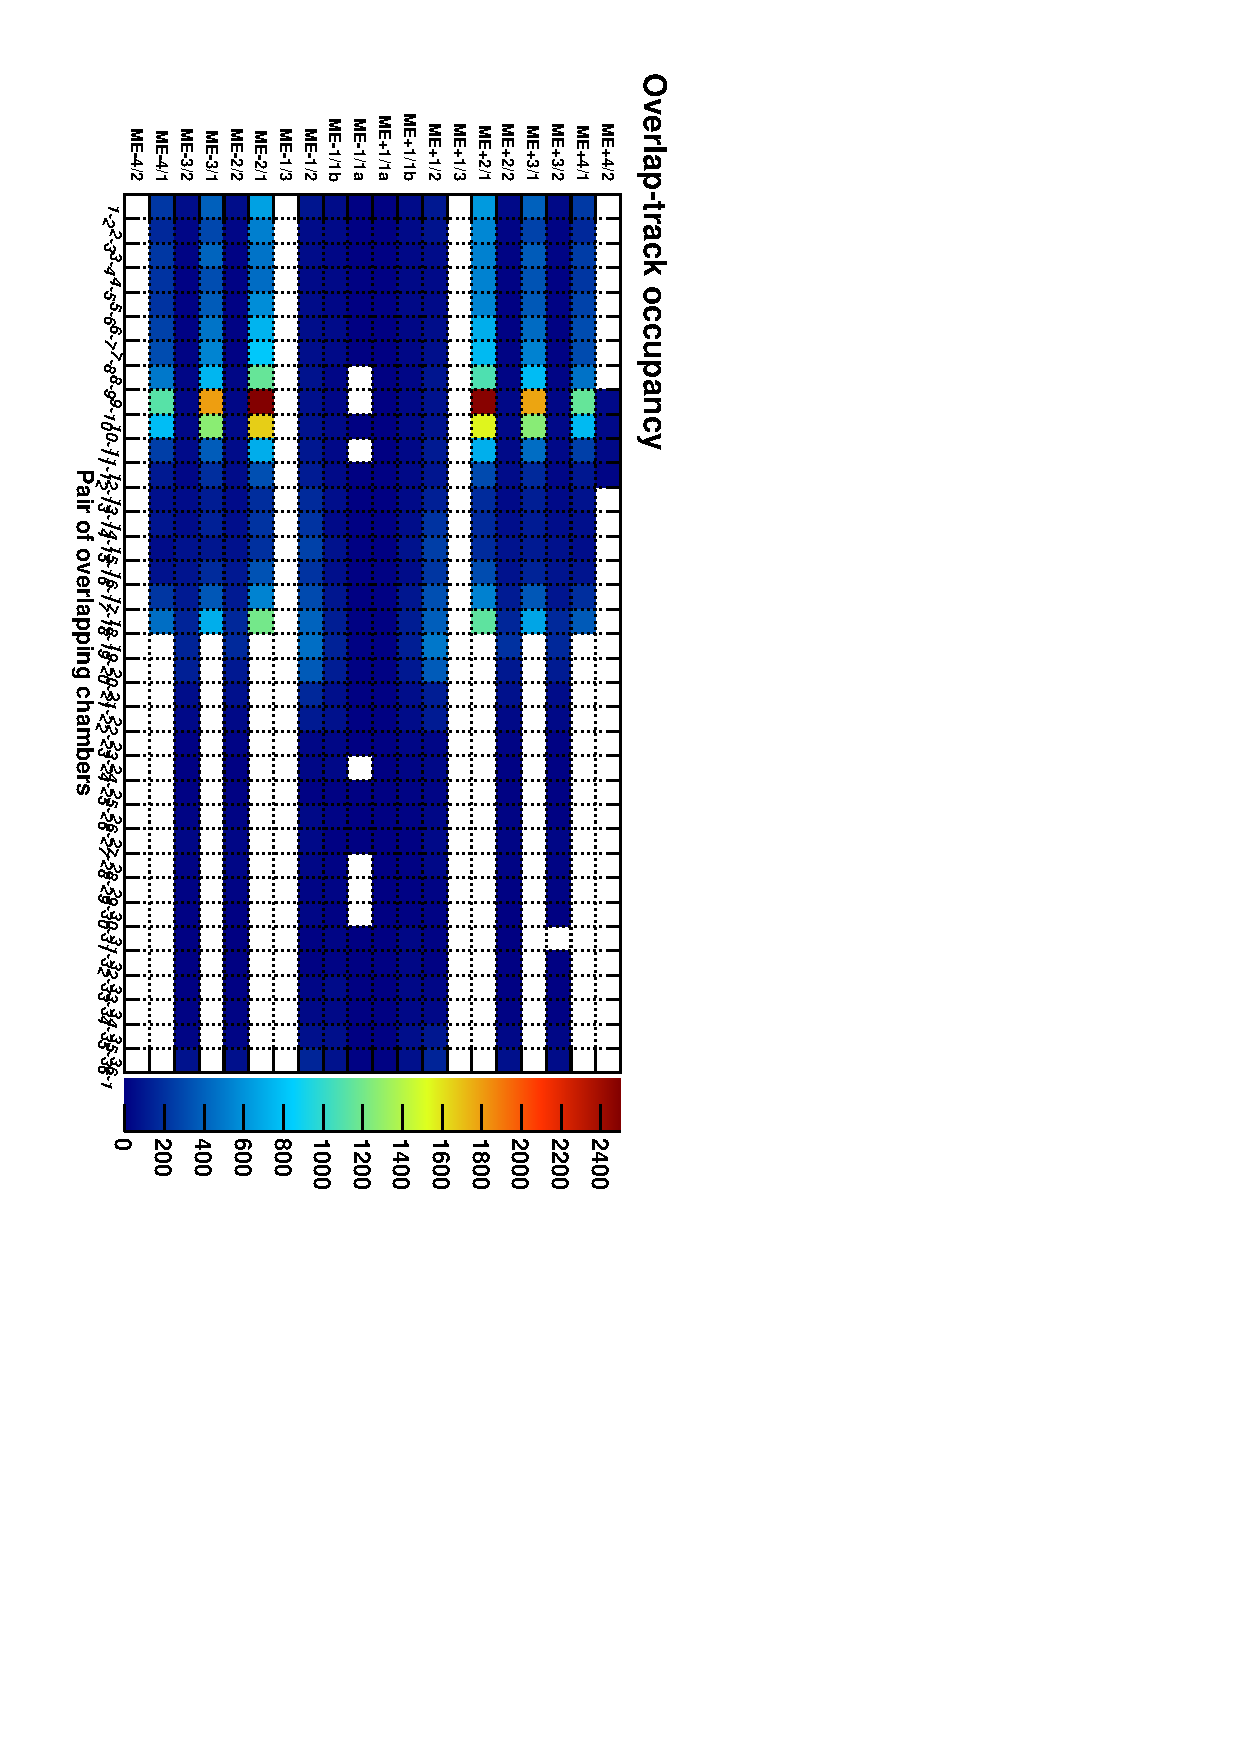
\includegraphics[height=\linewidth, angle=90]{occupancy1.pdf}}
\only<2>{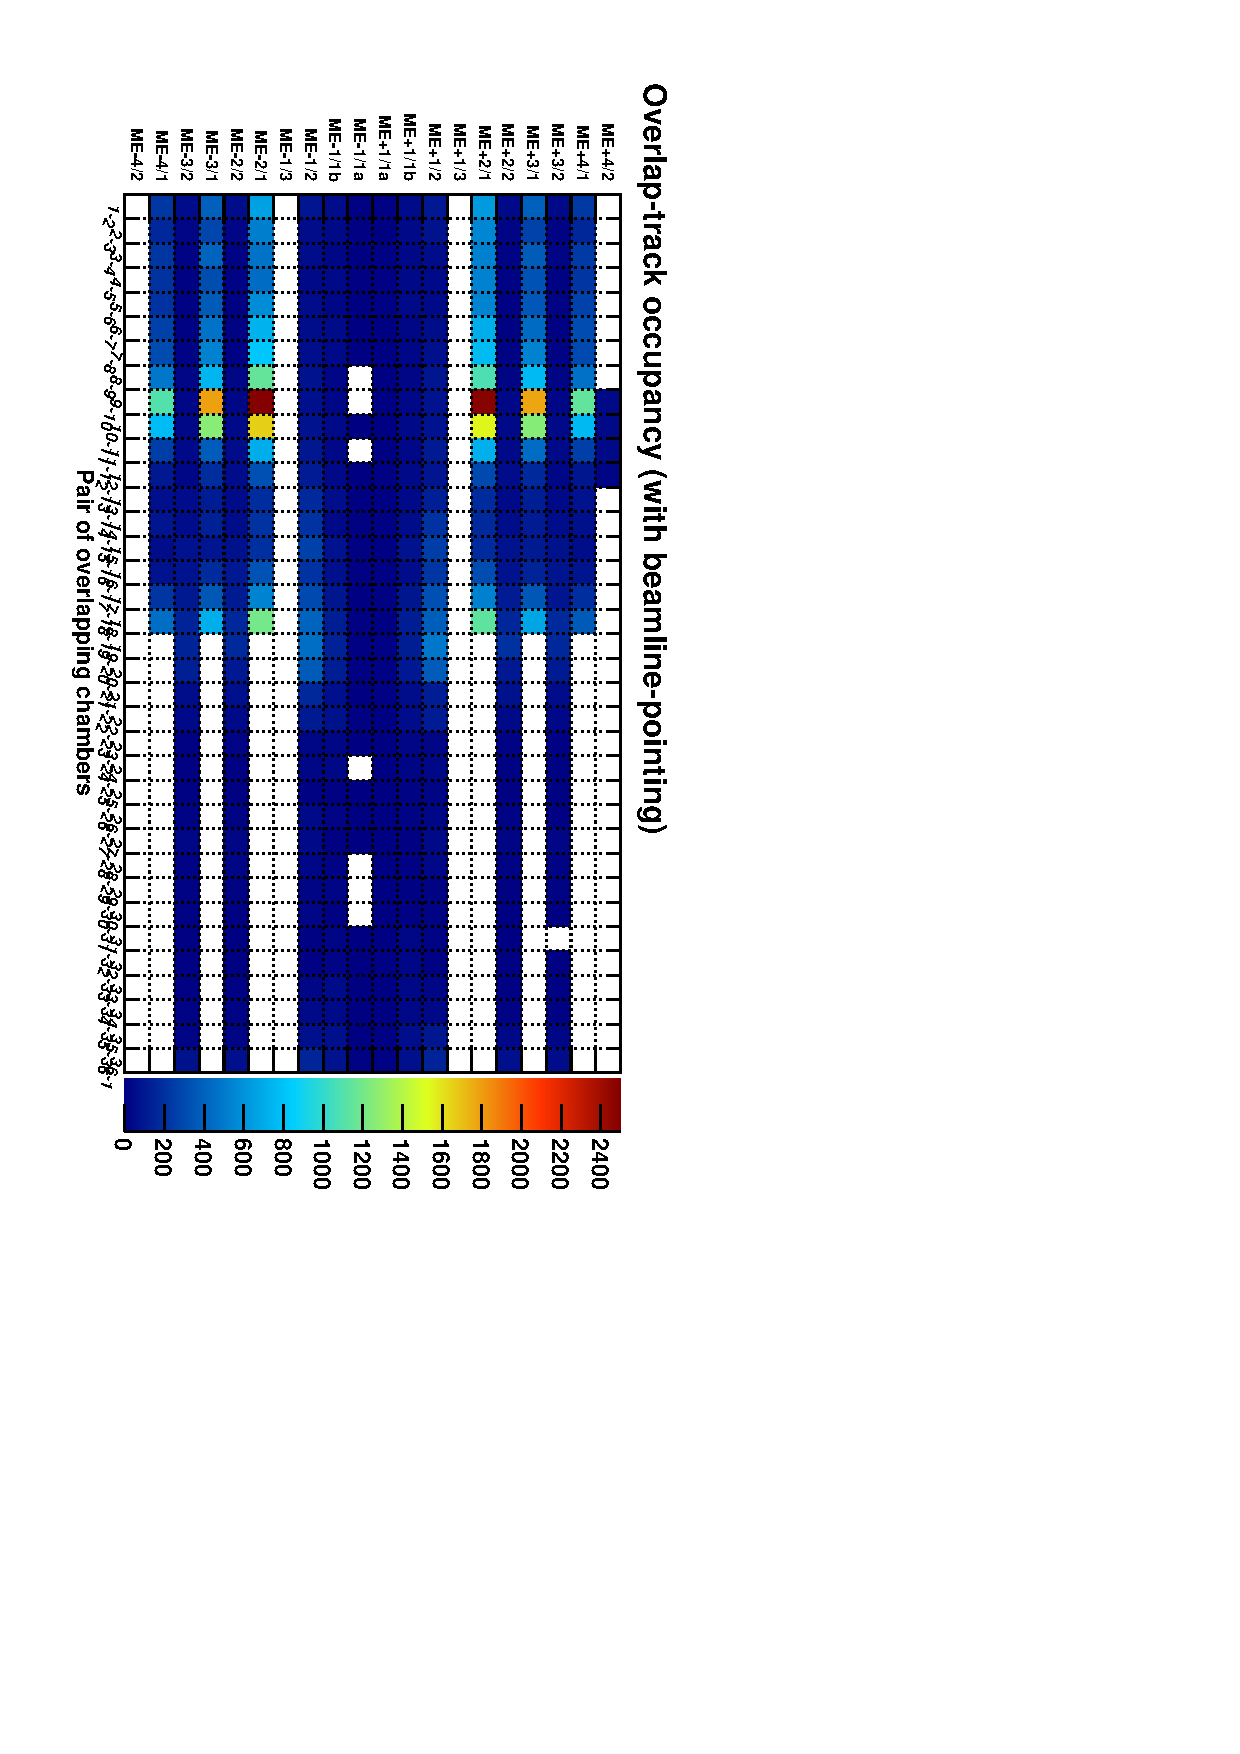
\includegraphics[height=\linewidth, angle=90]{occupancy2.pdf}}
\only<3>{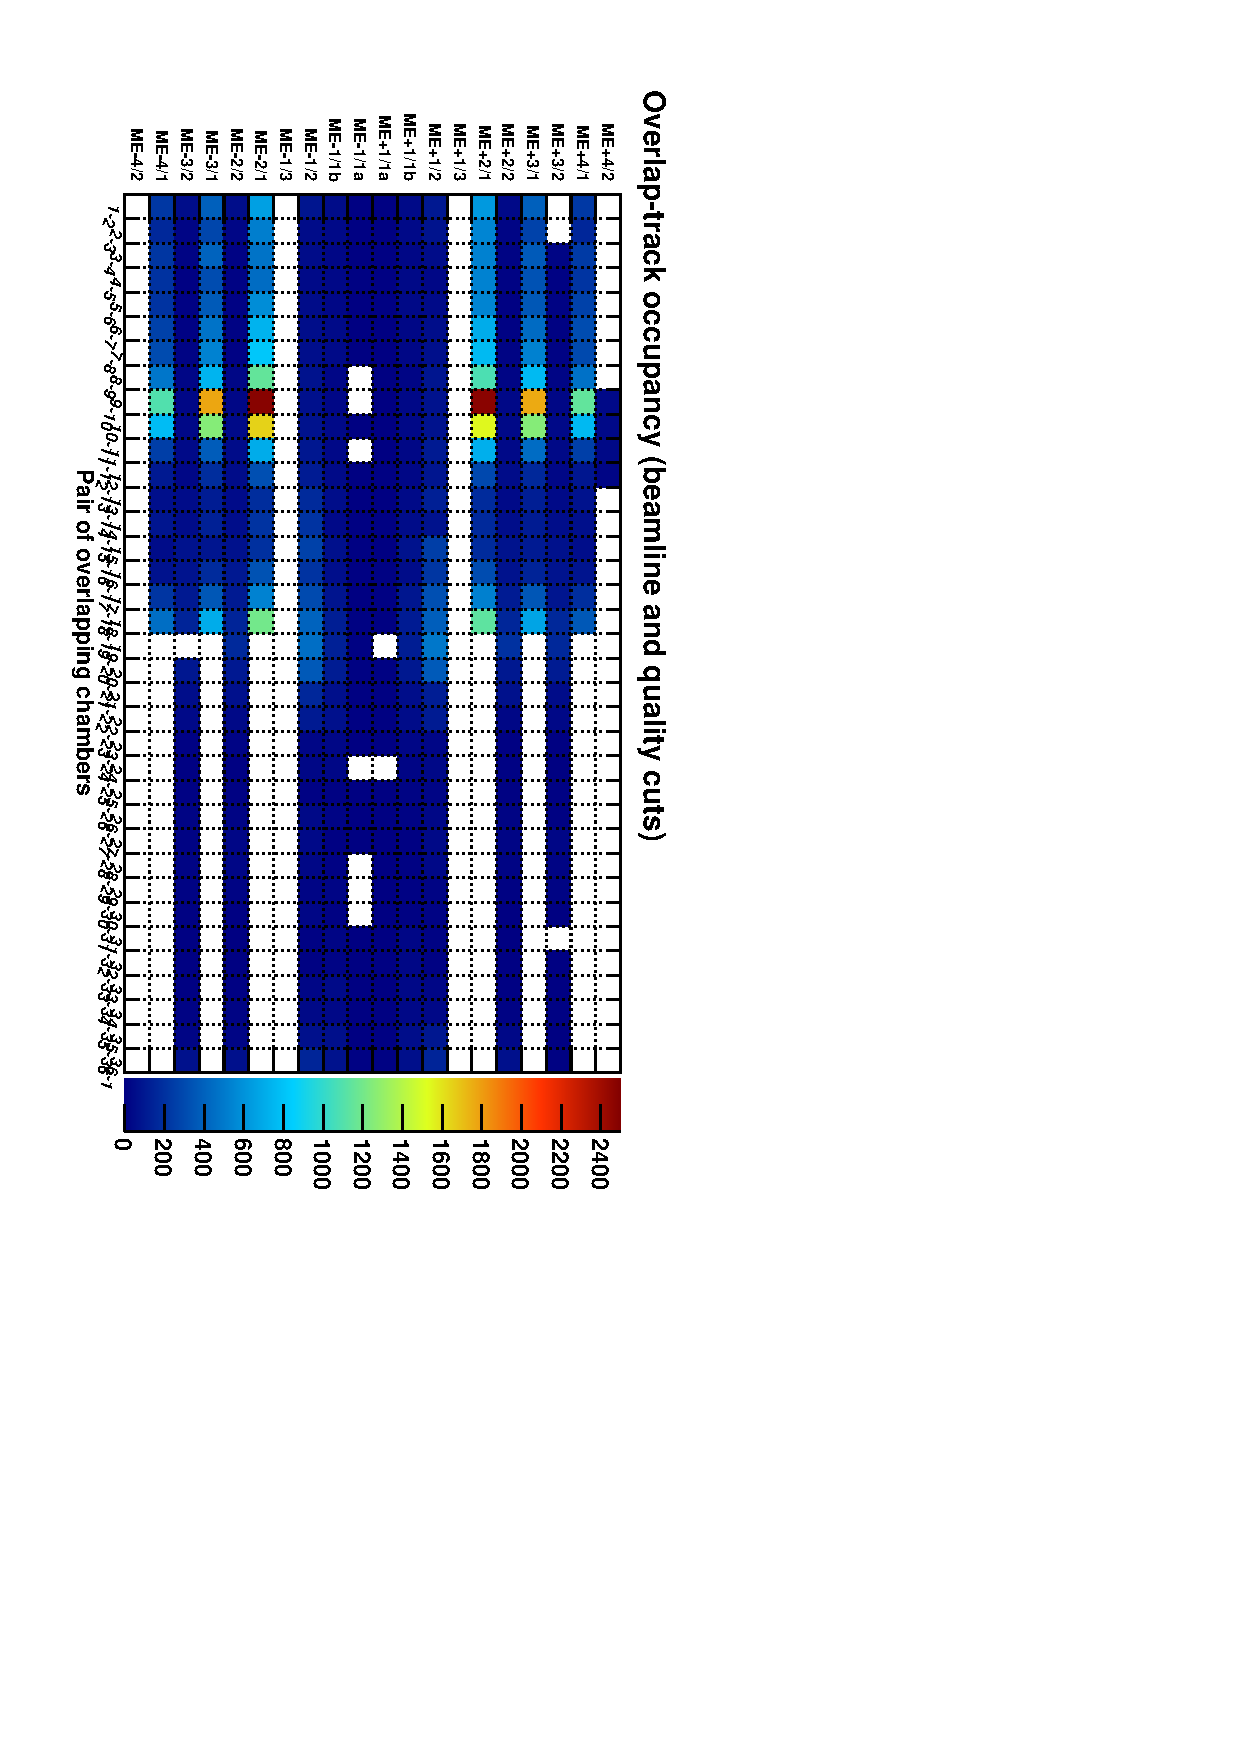
\includegraphics[height=\linewidth, angle=90]{occupancy3.pdf}}
\only<4>{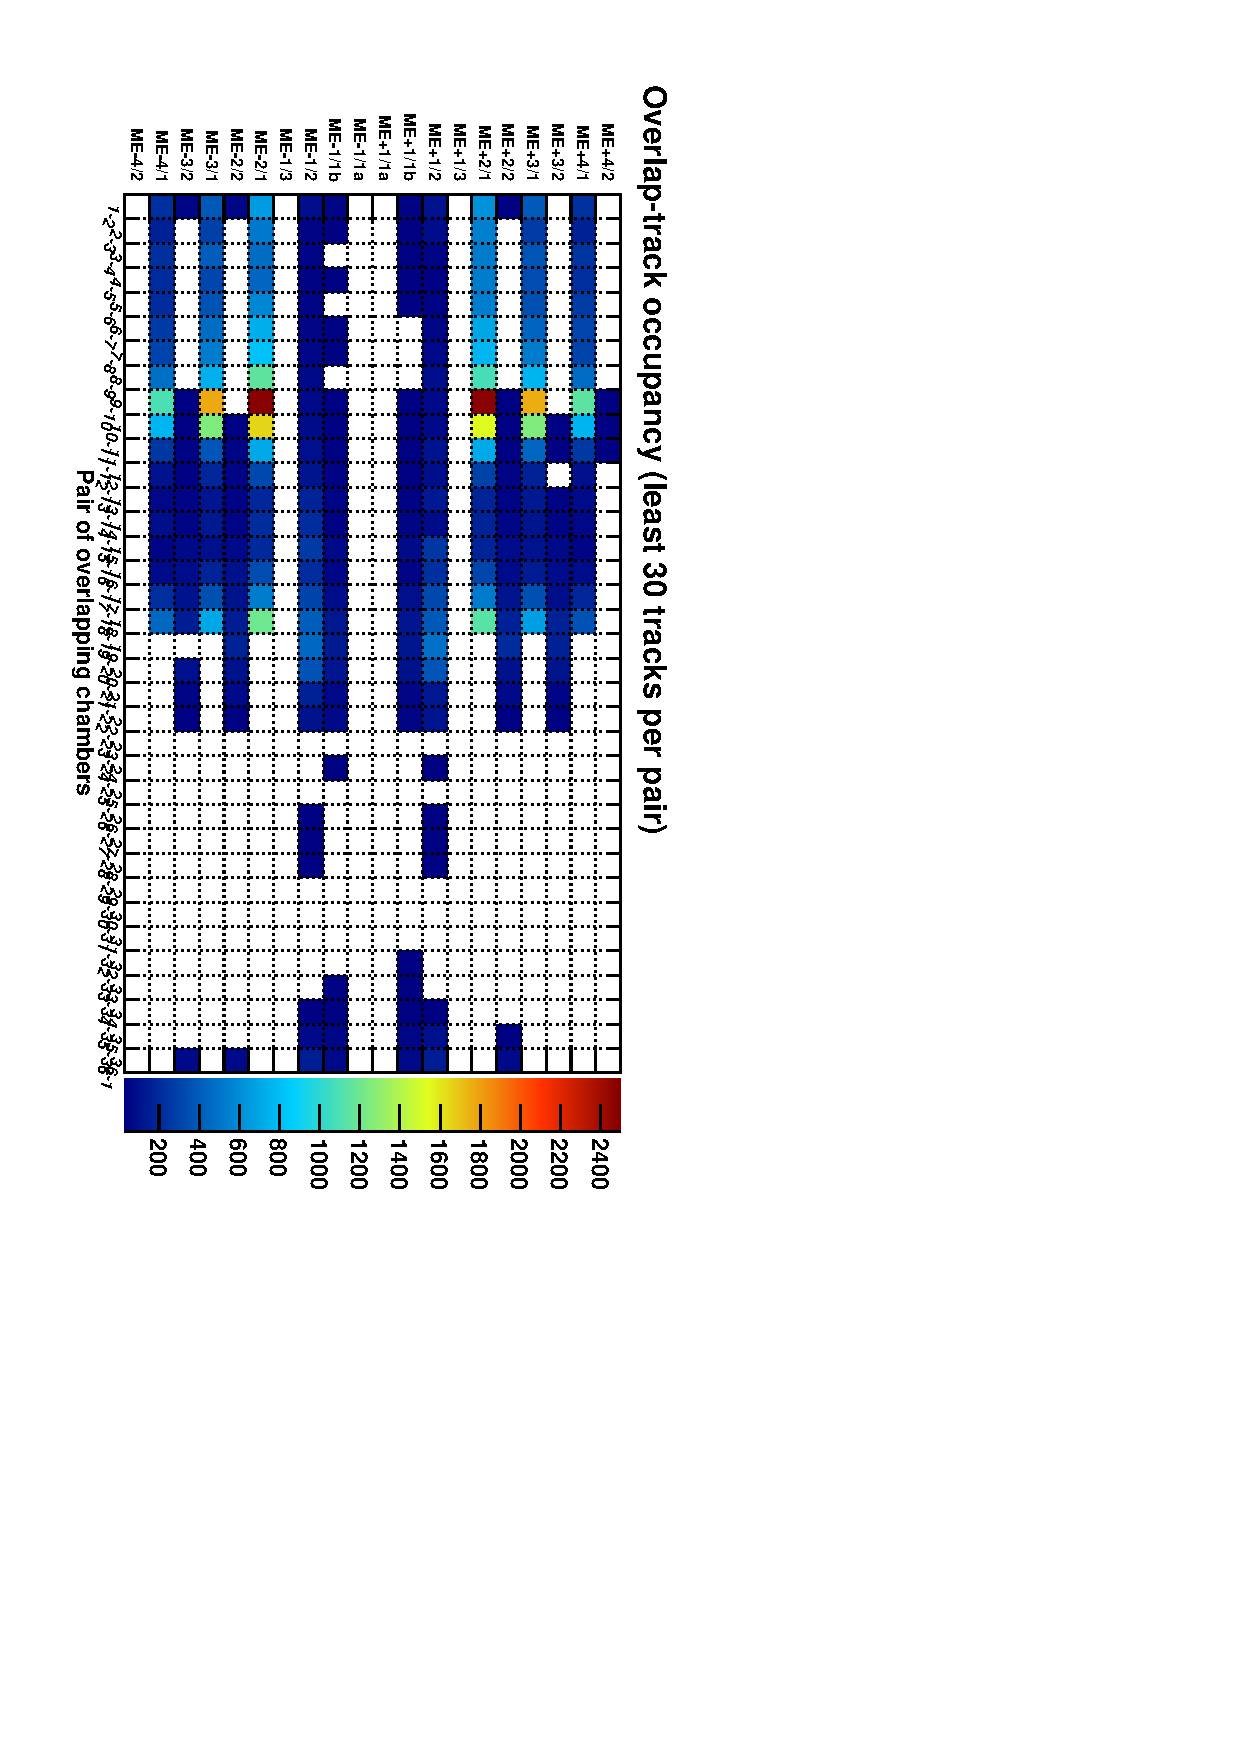
\includegraphics[height=\linewidth, angle=90]{occupancy4.pdf}}

\only<2>{\vspace{-6.7 cm} \hfill 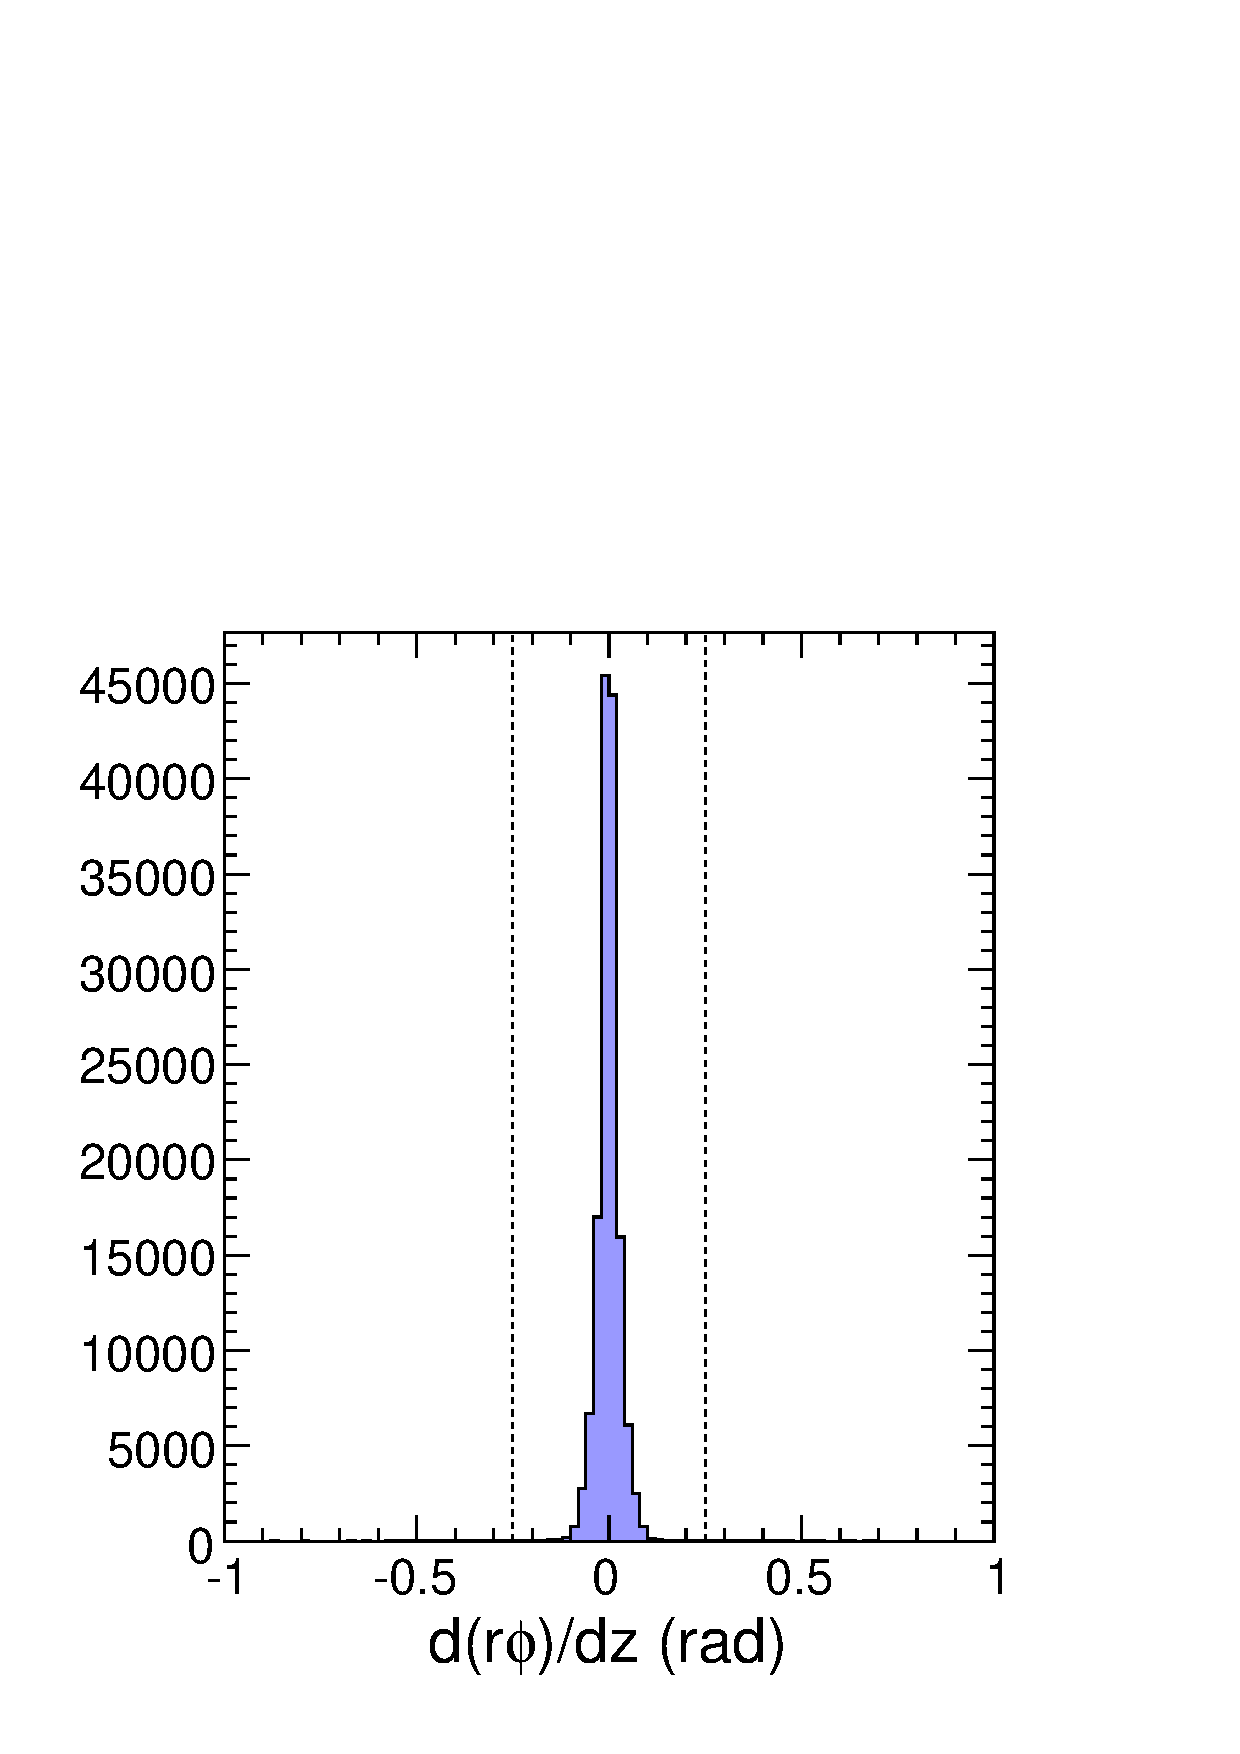
\includegraphics[height=3 cm]{beamline_pointing.pdf}}
\end{frame}

\begin{frame}
\frametitle{Global positions: $X$-$Y$}
\begin{itemize}
\item Global positions of accepted segments
\item Triggers (L1 and HLT) and offline selection do not explicitly select the overlapping strips \mbox{(they require activity in neighboring chambers)\hspace{-1 cm}}
\item The fact that we see radial spokes is a nice validation
\end{itemize}

\vfill
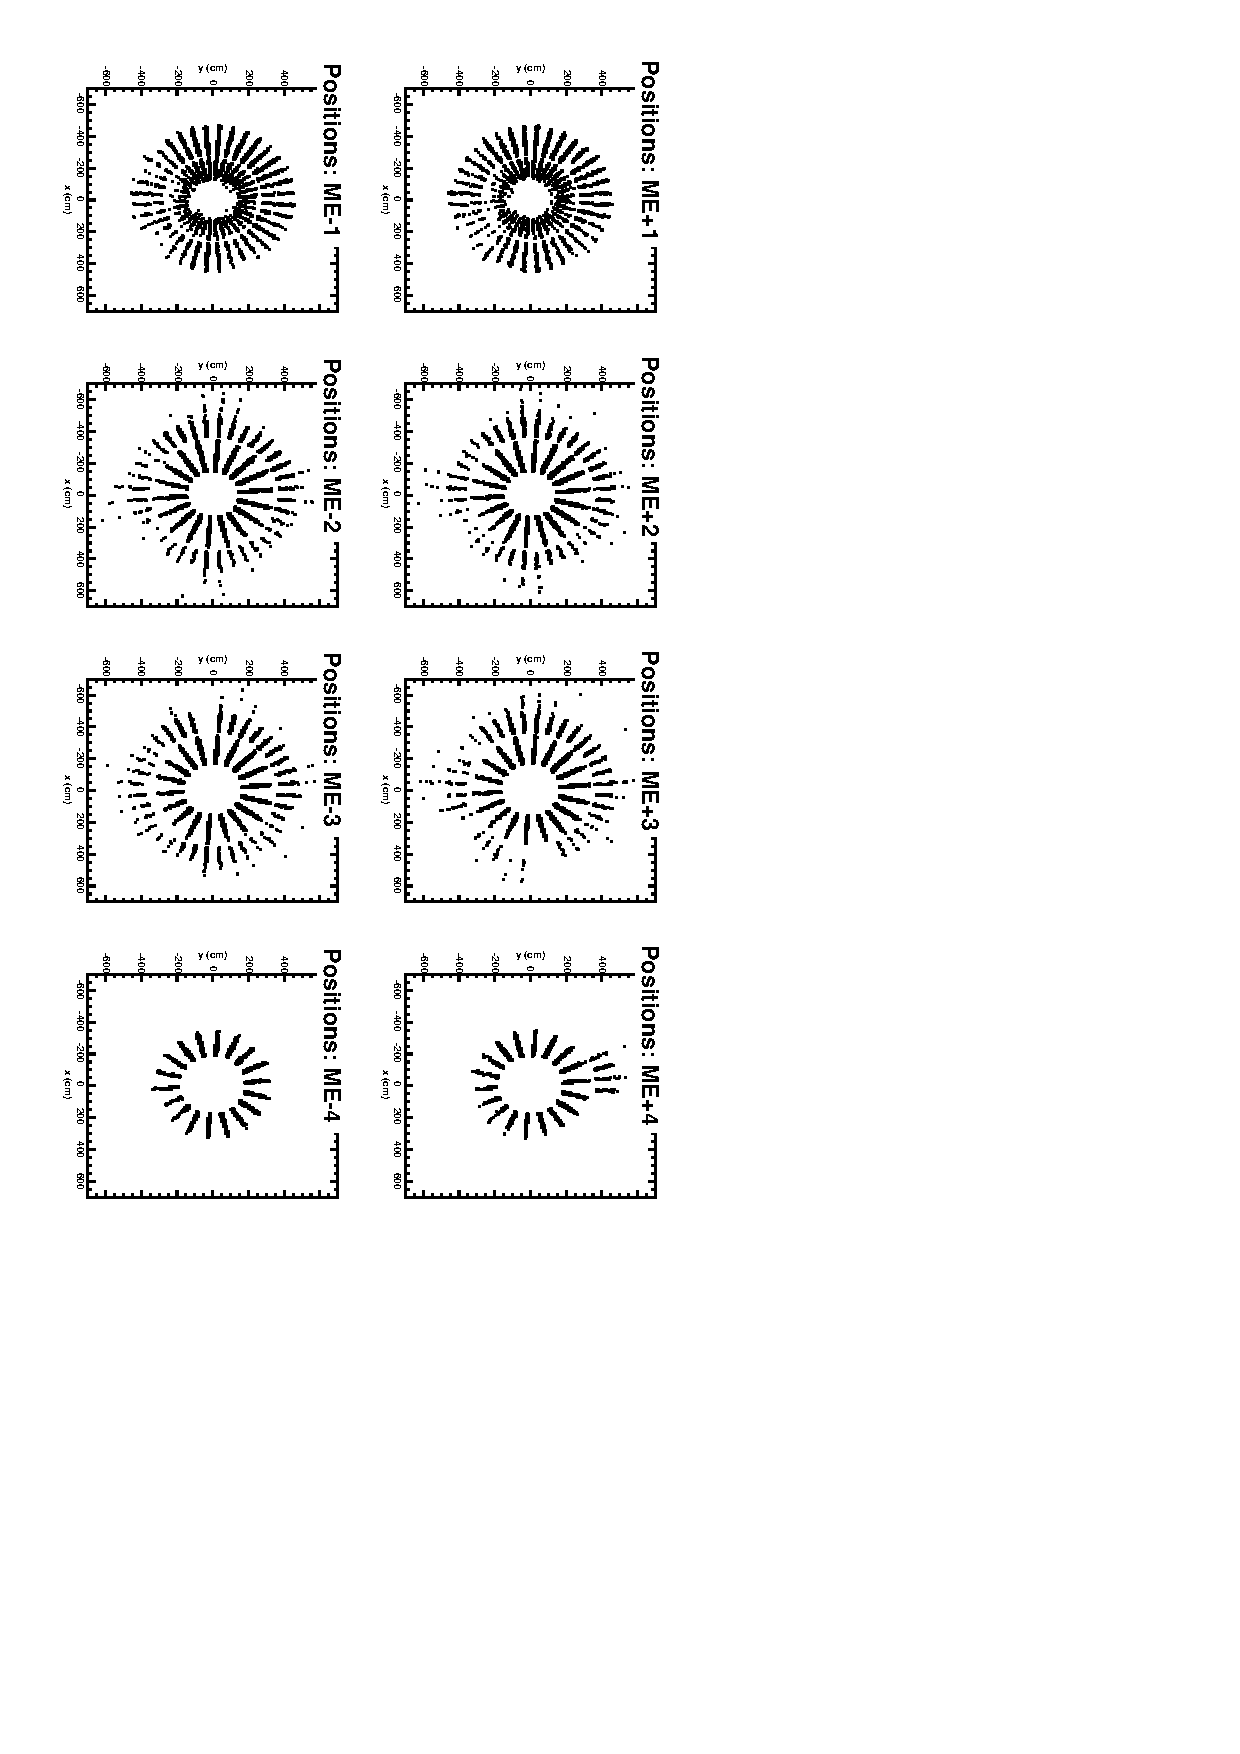
\includegraphics[height=\linewidth, angle=90]{positions1.pdf}
\end{frame}

\begin{frame}
\frametitle{Global positions: $R$-$\phi$}
\vspace{-0.75 cm}
\begin{columns}
\column{0.7\linewidth}
\vspace{0.5 cm}
\begin{itemize}
\item In the $R$-$\phi$ projection, we can see why ME1/1 (especially
  1/1a) has lower statistics: the triggers are coming from ME2 and ME3
\item I'm trying to find out if there are other trigger lines which would
  illuminate this better
\end{itemize}

\column{0.3\linewidth}
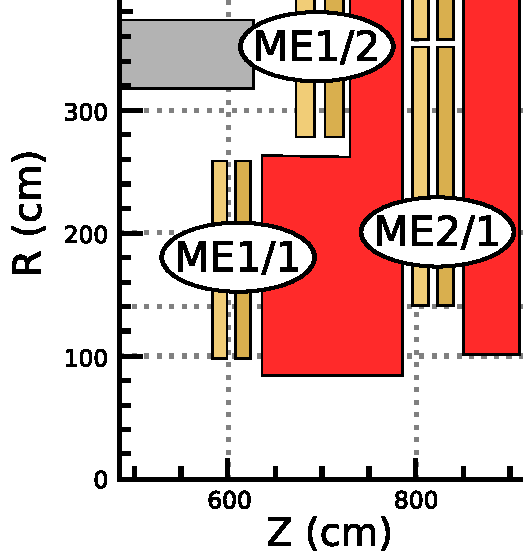
\includegraphics[width=\linewidth]{geometry_me1_me2.pdf}
\end{columns}

\vfill
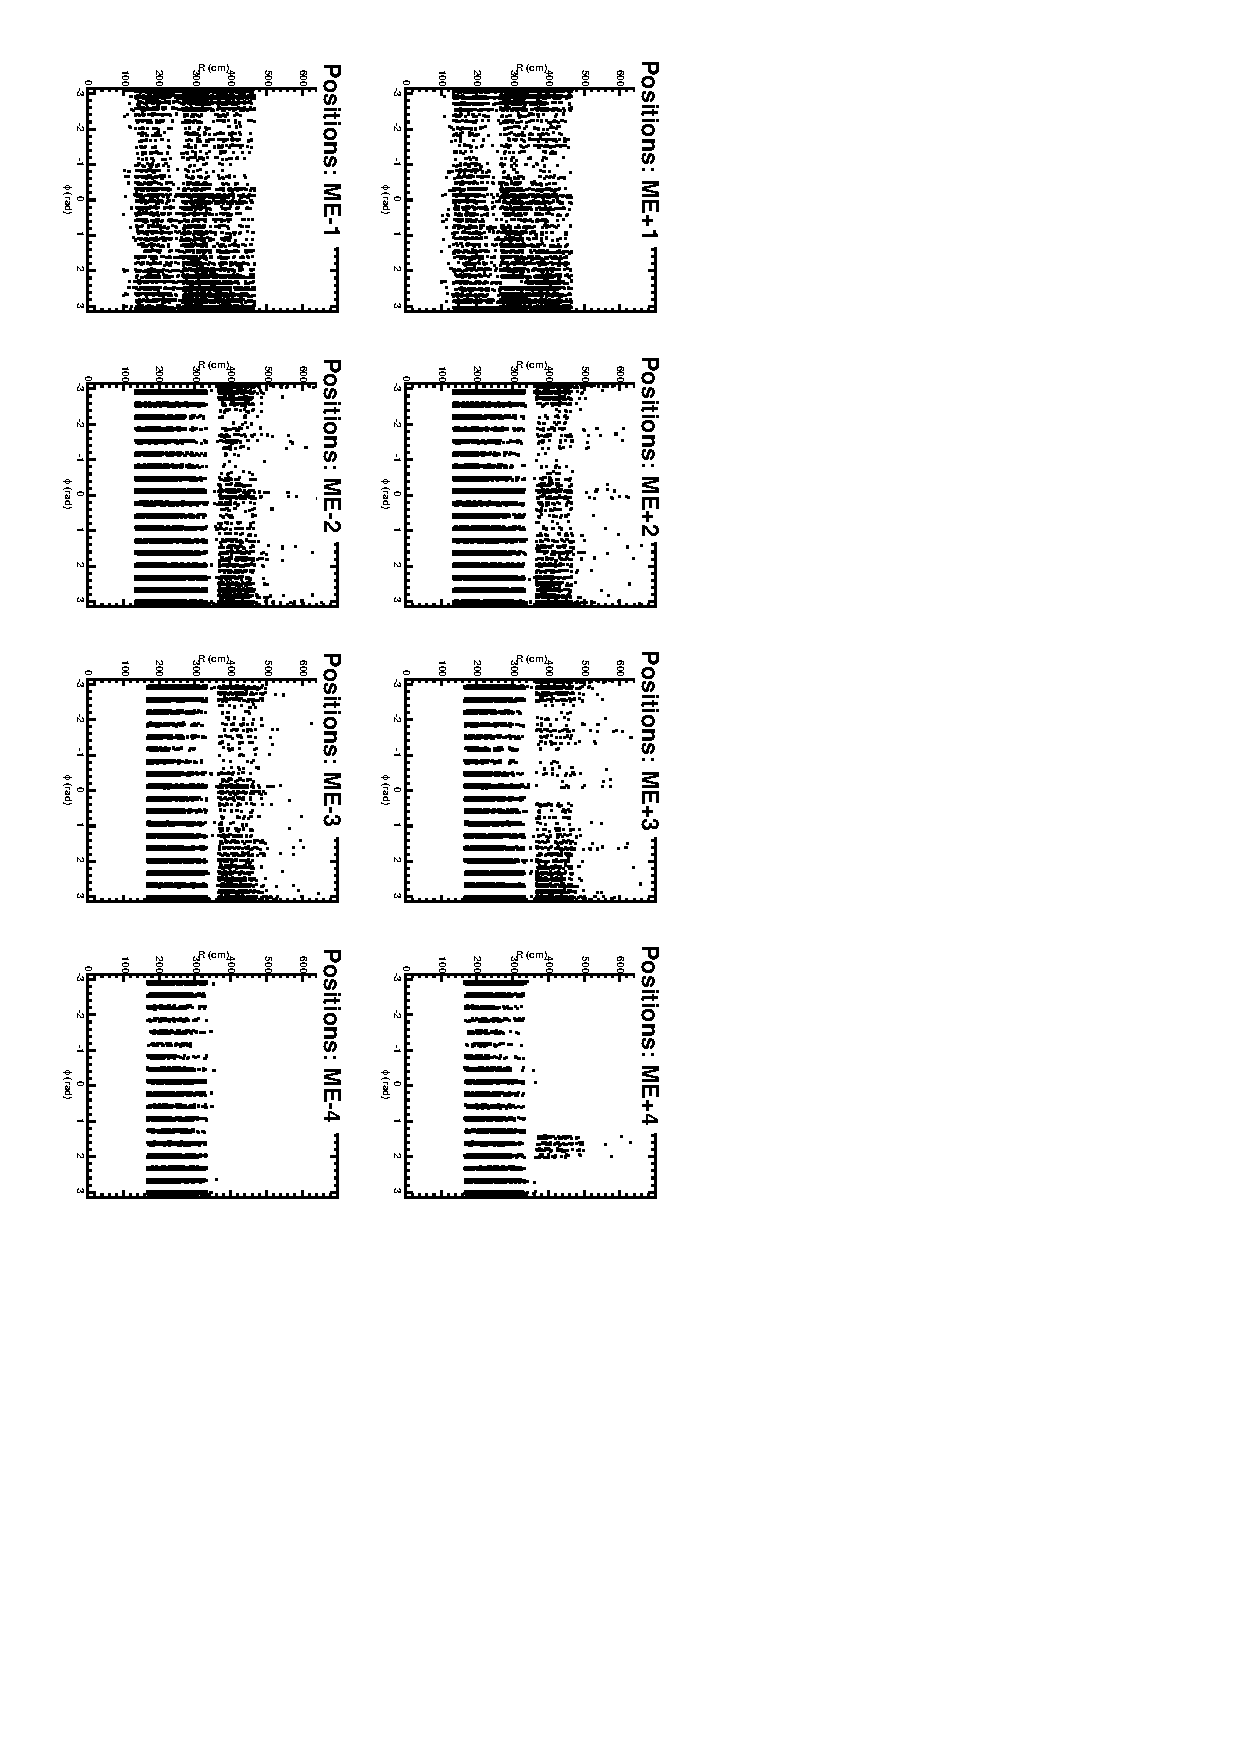
\includegraphics[height=\linewidth, angle=90]{positions2.pdf}
\end{frame}

\begin{frame}
\frametitle{Reminder of method}
\begin{columns}
\column{0.6\linewidth}
\begin{itemize}\setlength{\itemsep}{0.25 cm}
\item Single muon passing through overlap region leaves segments in two neighboring chambers 
\item Any discrepancies in segment slopes $\Delta \frac{d(r\phi)}{dz}$ or intercepts at a plane between the chambers $\Delta (r\phi)$ imply relative corrections to $\delta_{\phi_y}$, $\delta_{r\phi}$, and $\delta_{\phi_z}$
\item Propagate corrections around the ring by solving a system of equations
\item $\delta_{\phi_y}$, $\delta_{r\phi}$, and $\delta_{\phi_z}$ can be solved independently, as long as they are done in that order
\end{itemize}
\column{0.4\linewidth}
\begin{center}
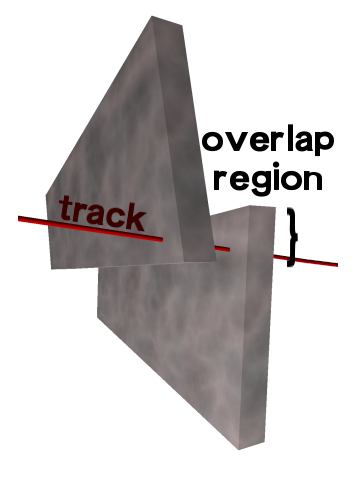
\includegraphics[width=0.45\linewidth]{overlaps.png}

\vspace{0.5 cm}
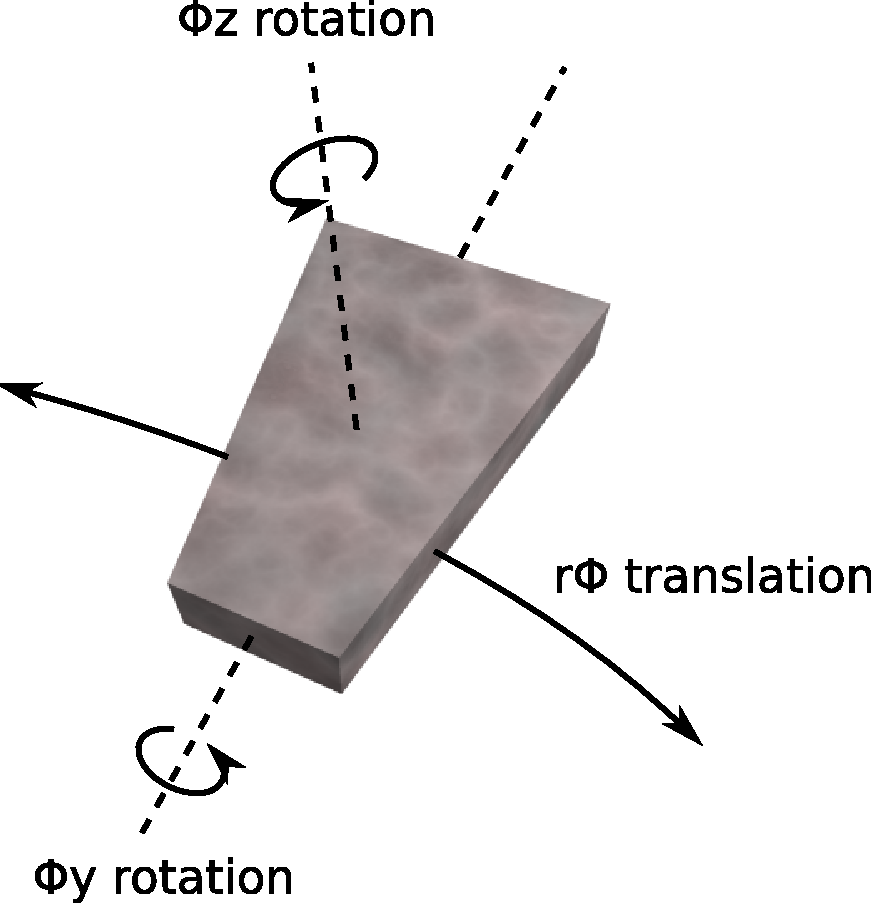
\includegraphics[width=\linewidth]{csc_coordinates.pdf}
\end{center}
\end{columns}
\end{frame}

\begin{frame}
\frametitle{Alignment of ME2/1, 3/1, 4/1}

\vfill
\begin{columns}
\column{0.7\linewidth}
\textcolor{darkblue}{Step 1: align $\phi_y$ (left)}
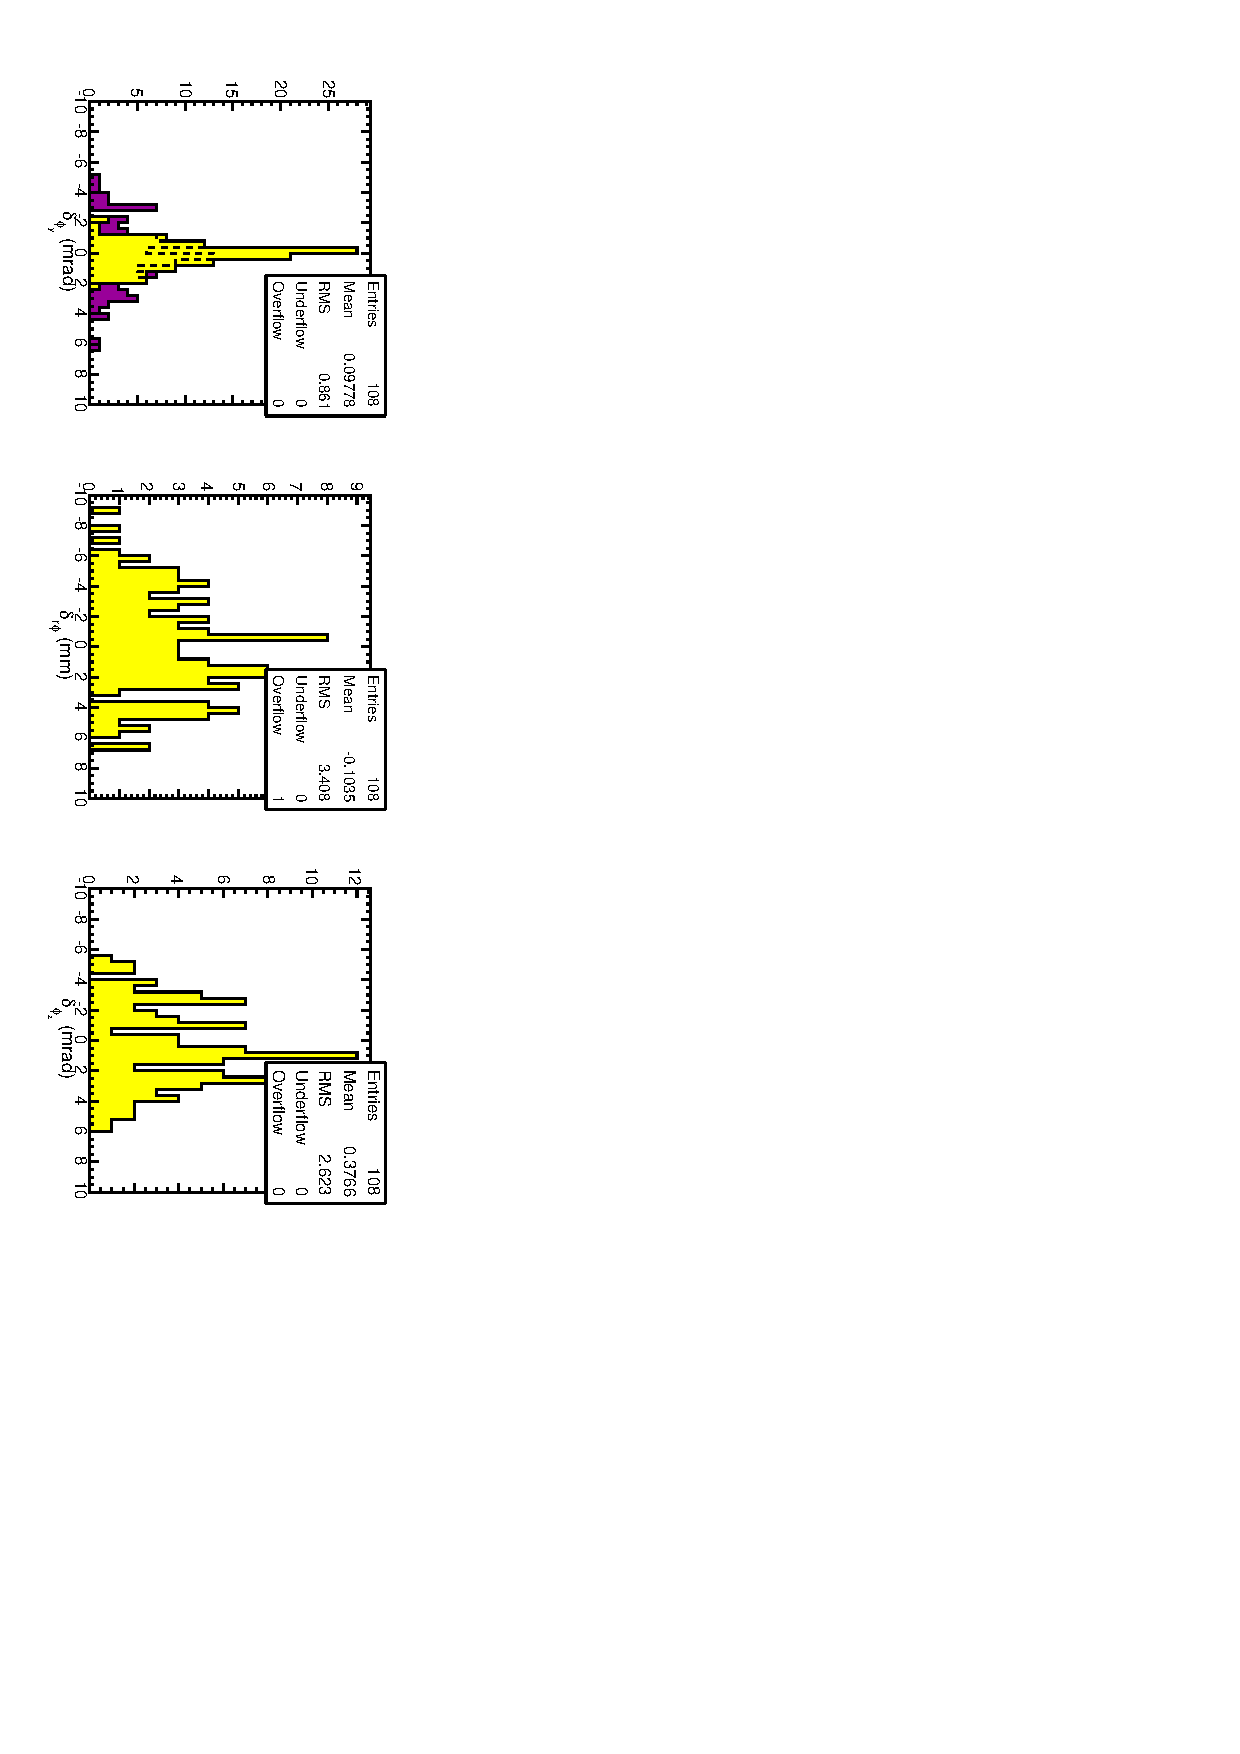
\includegraphics[height=\linewidth, angle=90]{align_step1.pdf}

\textcolor{darkblue}{Step 2: align $r\phi$ (middle)}
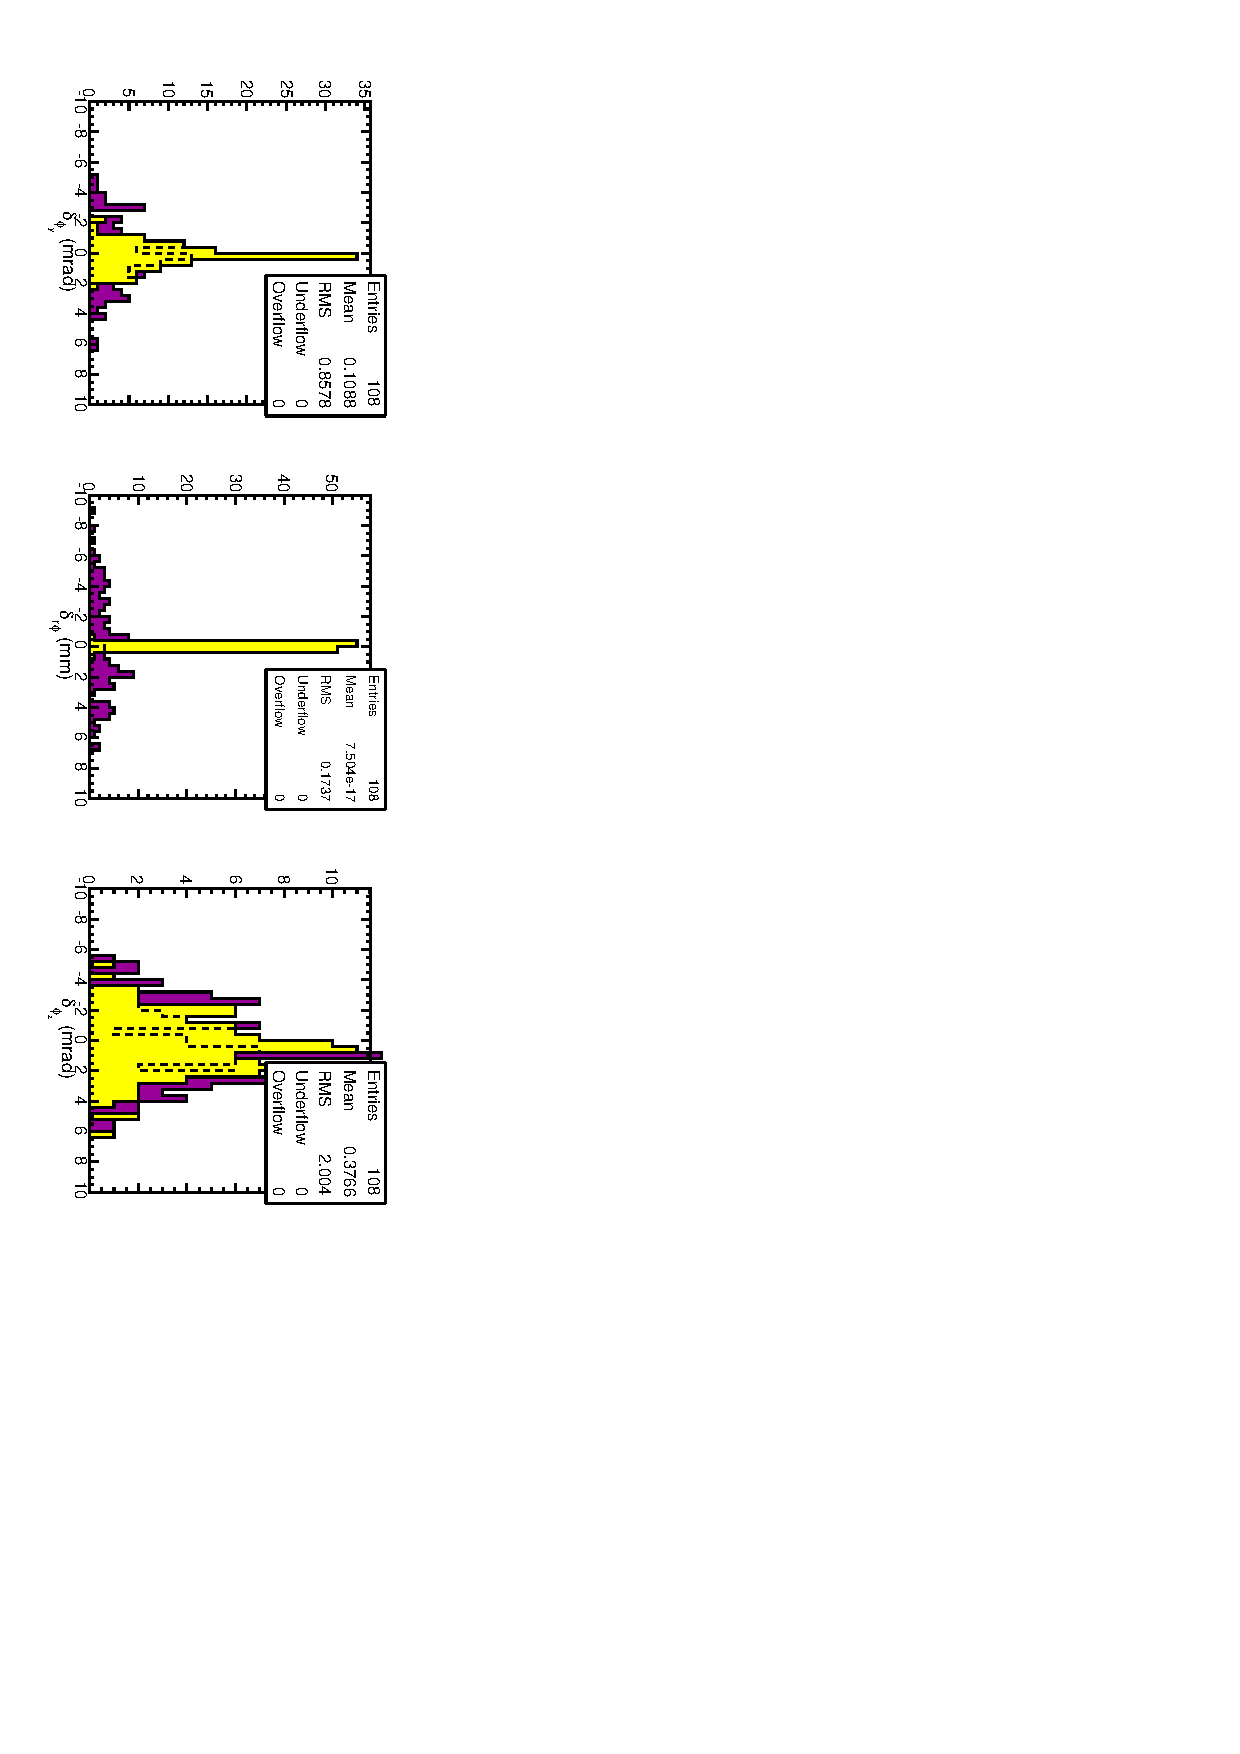
\includegraphics[height=\linewidth, angle=90]{align_step2.pdf}

\textcolor{darkblue}{Step 3: align $\phi_z$ (right)}
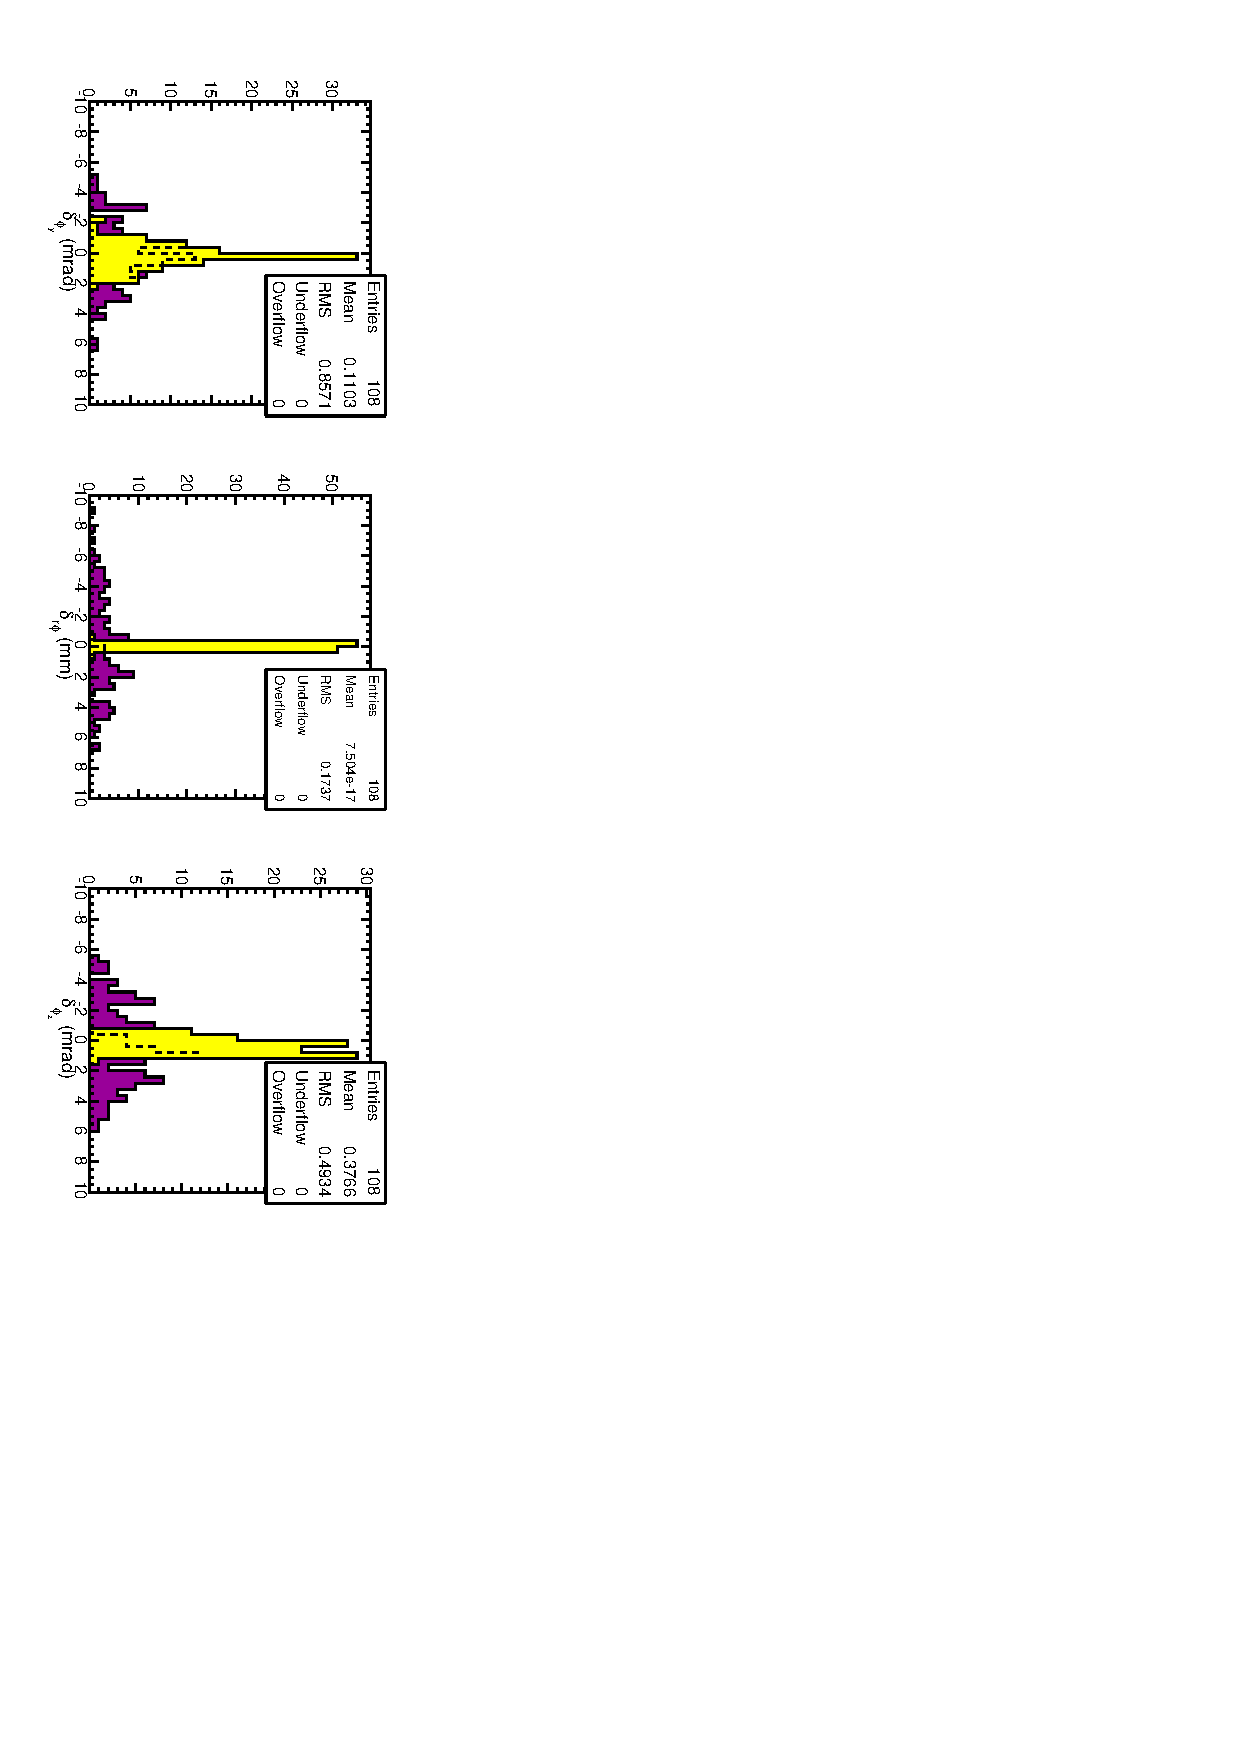
\includegraphics[height=\linewidth, angle=90]{align_step3.pdf}
\column{0.3\linewidth}

\begin{itemize}
\item Differences between aligned and \mbox{true chamber\hspace{-0.5 cm}} parameters (2/1, 3/1, 4/1 only)

\item Rotation of whole ring in $r\phi$ removed

\item Purple: before \\ Yellow: after

\item Final resolution \\ $\phi_y$: 0.85~mrad \\ $r\phi$: 0.17~mm \\ $\phi_z$: 0.49~mrad

\item \mbox{Depends on MC $R$\hspace{-1 cm}} \\ and \mbox{$\phi$ distributions;\hspace{-1 cm}} \\ not realistic!
\end{itemize}
\end{columns}
\end{frame}

\begin{frame}
\frametitle{Independence of parameters}

\textcolor{darkblue}{Step 3 (previous page)}
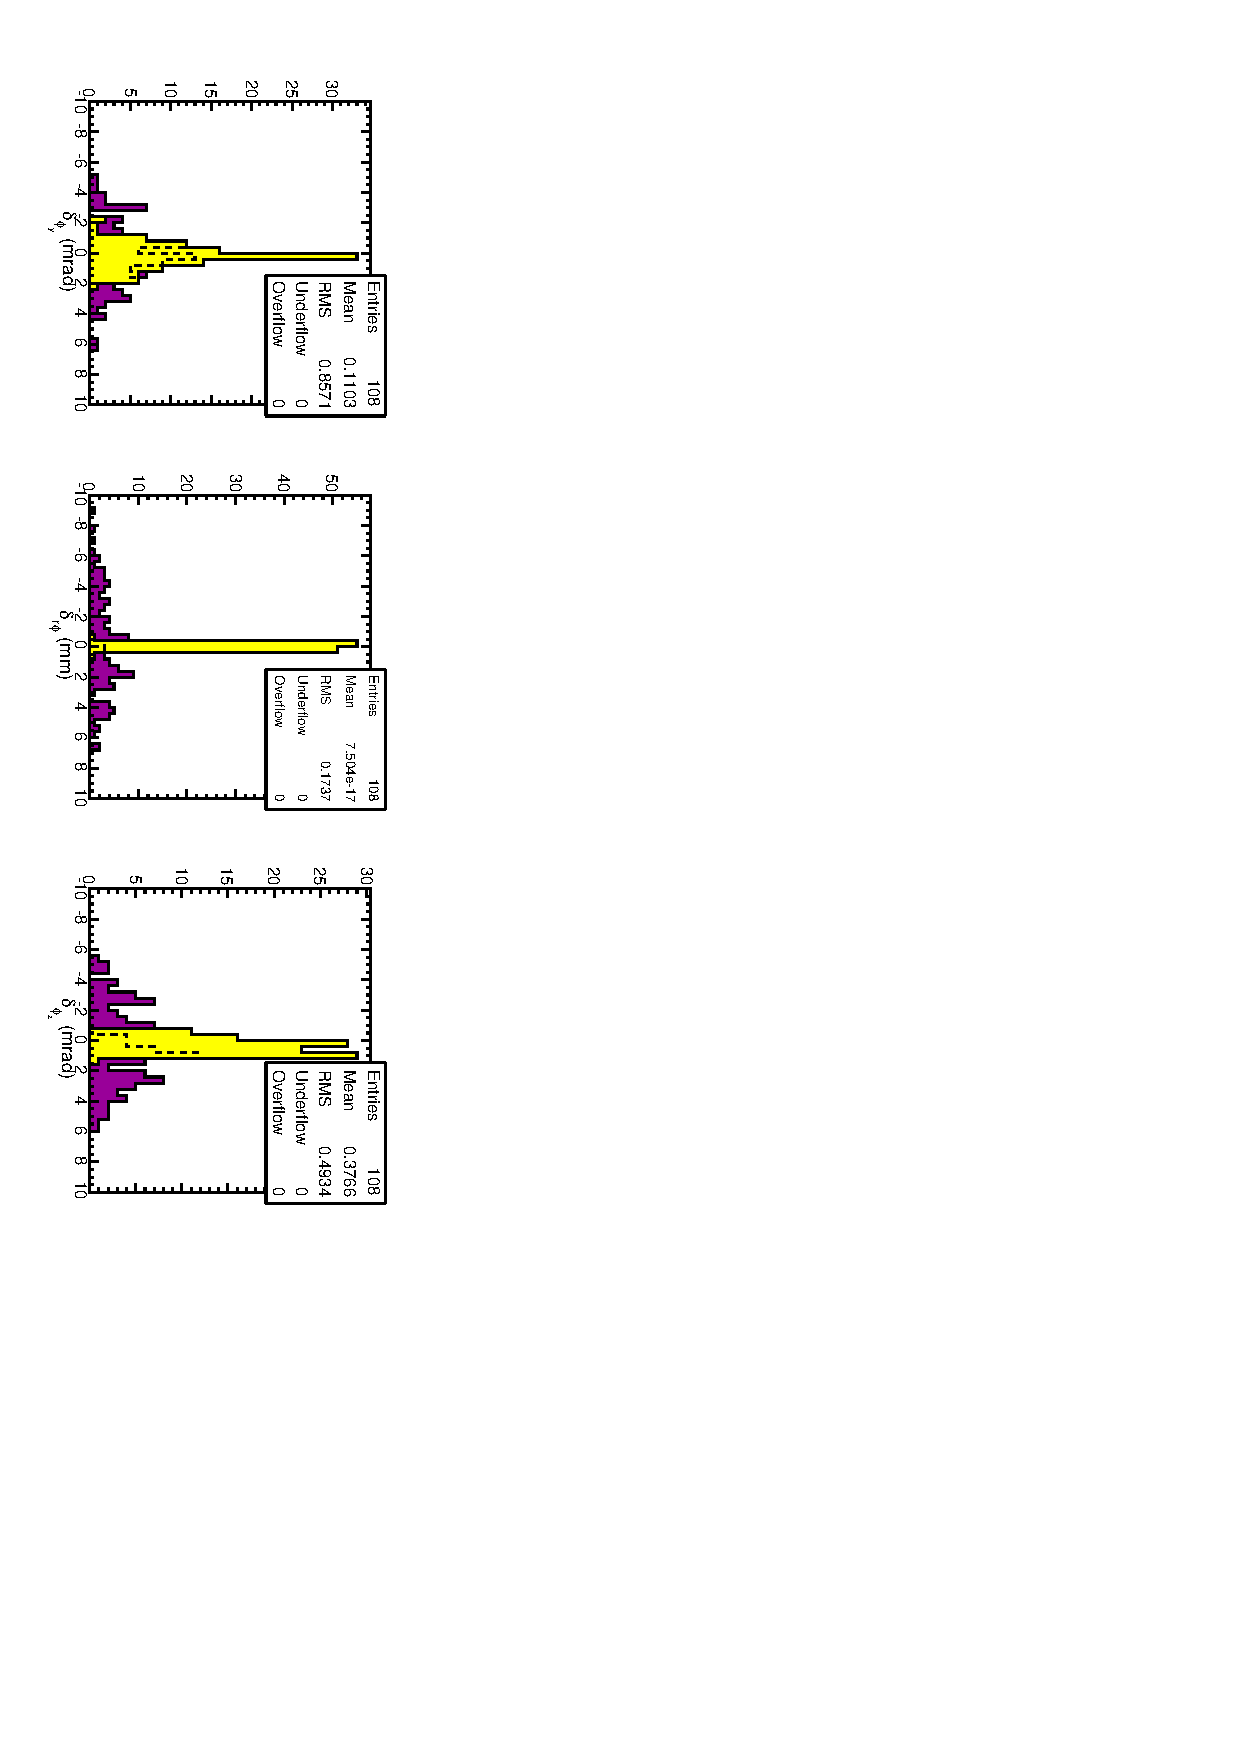
\includegraphics[height=\linewidth, angle=90]{align_step3.pdf}

\textcolor{darkblue}{\mbox{Step 6: repeated everything, to allow for any interdependence of parameters\hspace{-1 cm}}}
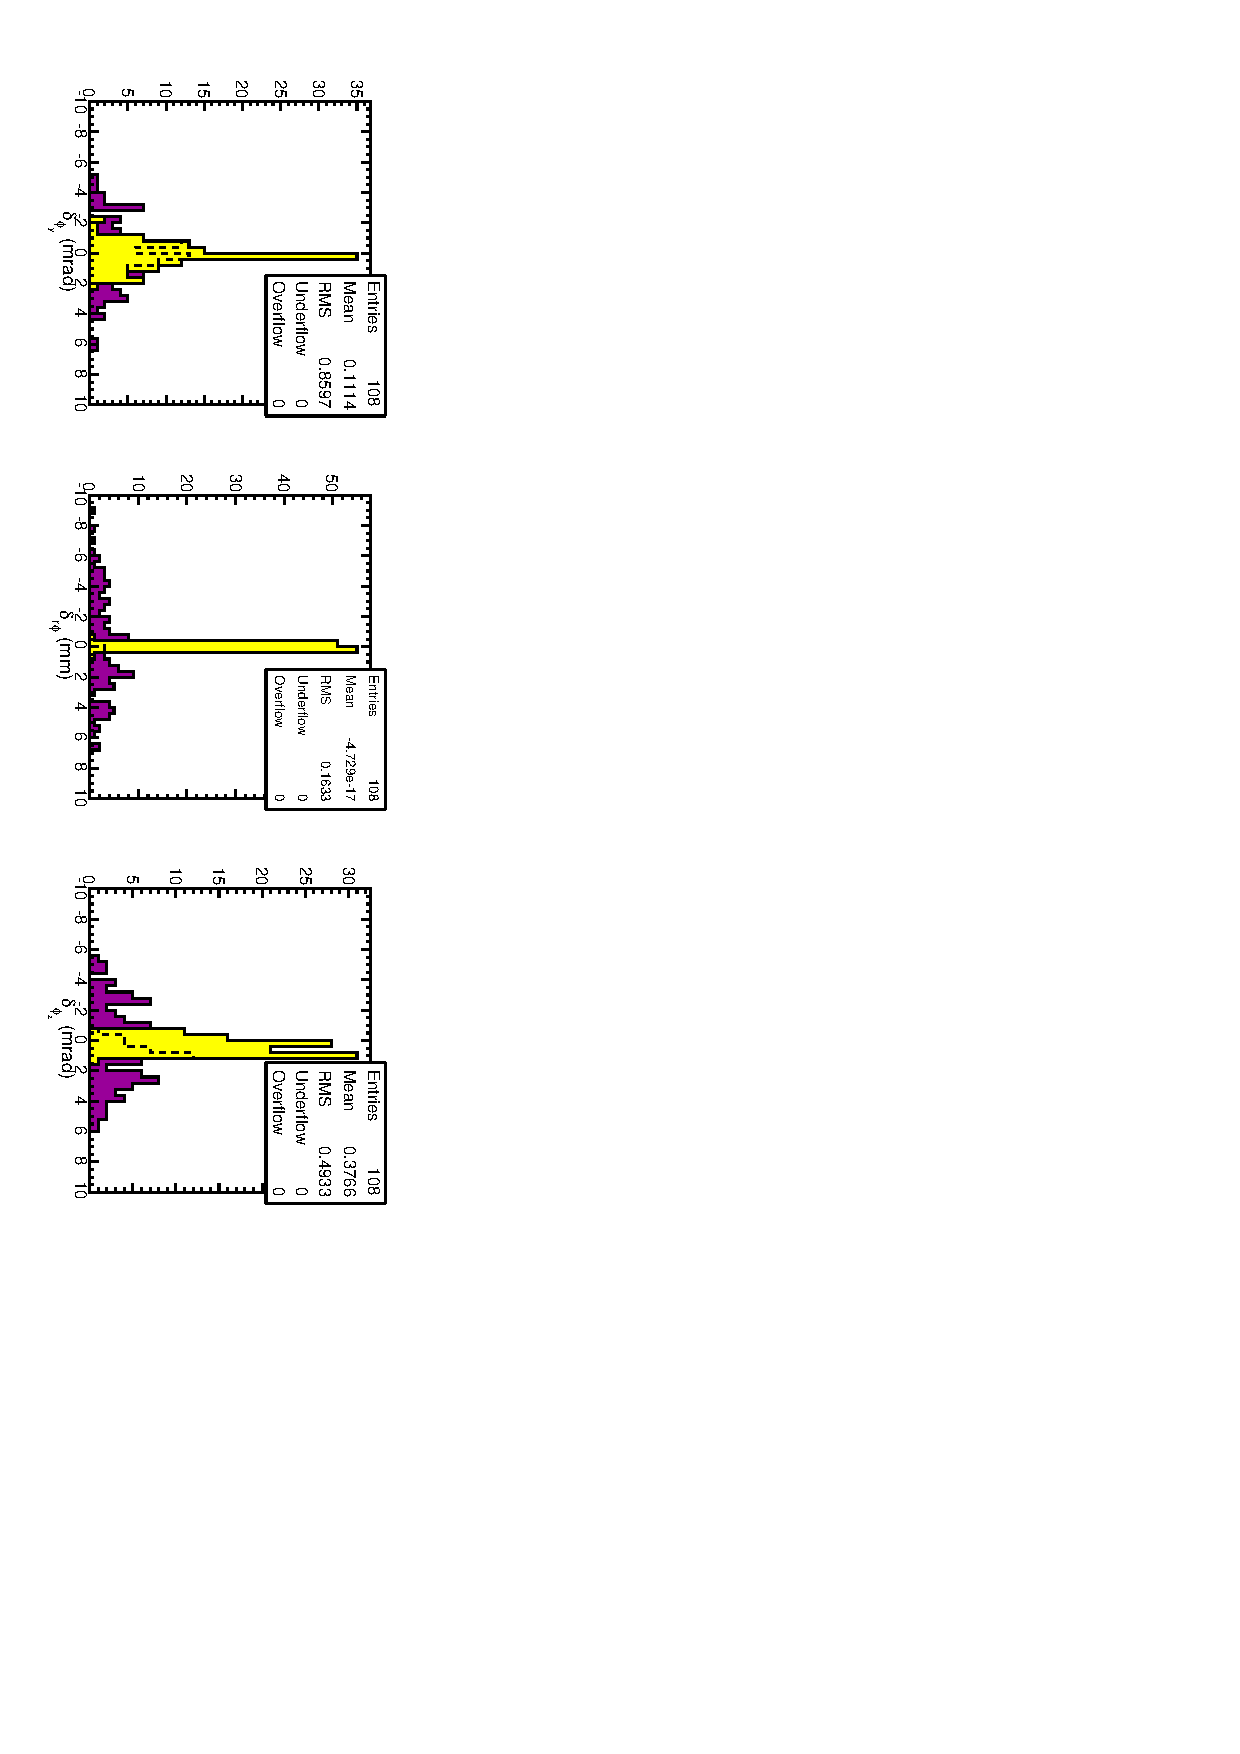
\includegraphics[height=\linewidth, angle=90]{align_step4.pdf}

\vspace{-0.25 cm}
\begin{itemize}
\item No significant change
\end{itemize}
\end{frame}

\begin{frame}
\frametitle{Residuals}
\begin{center}
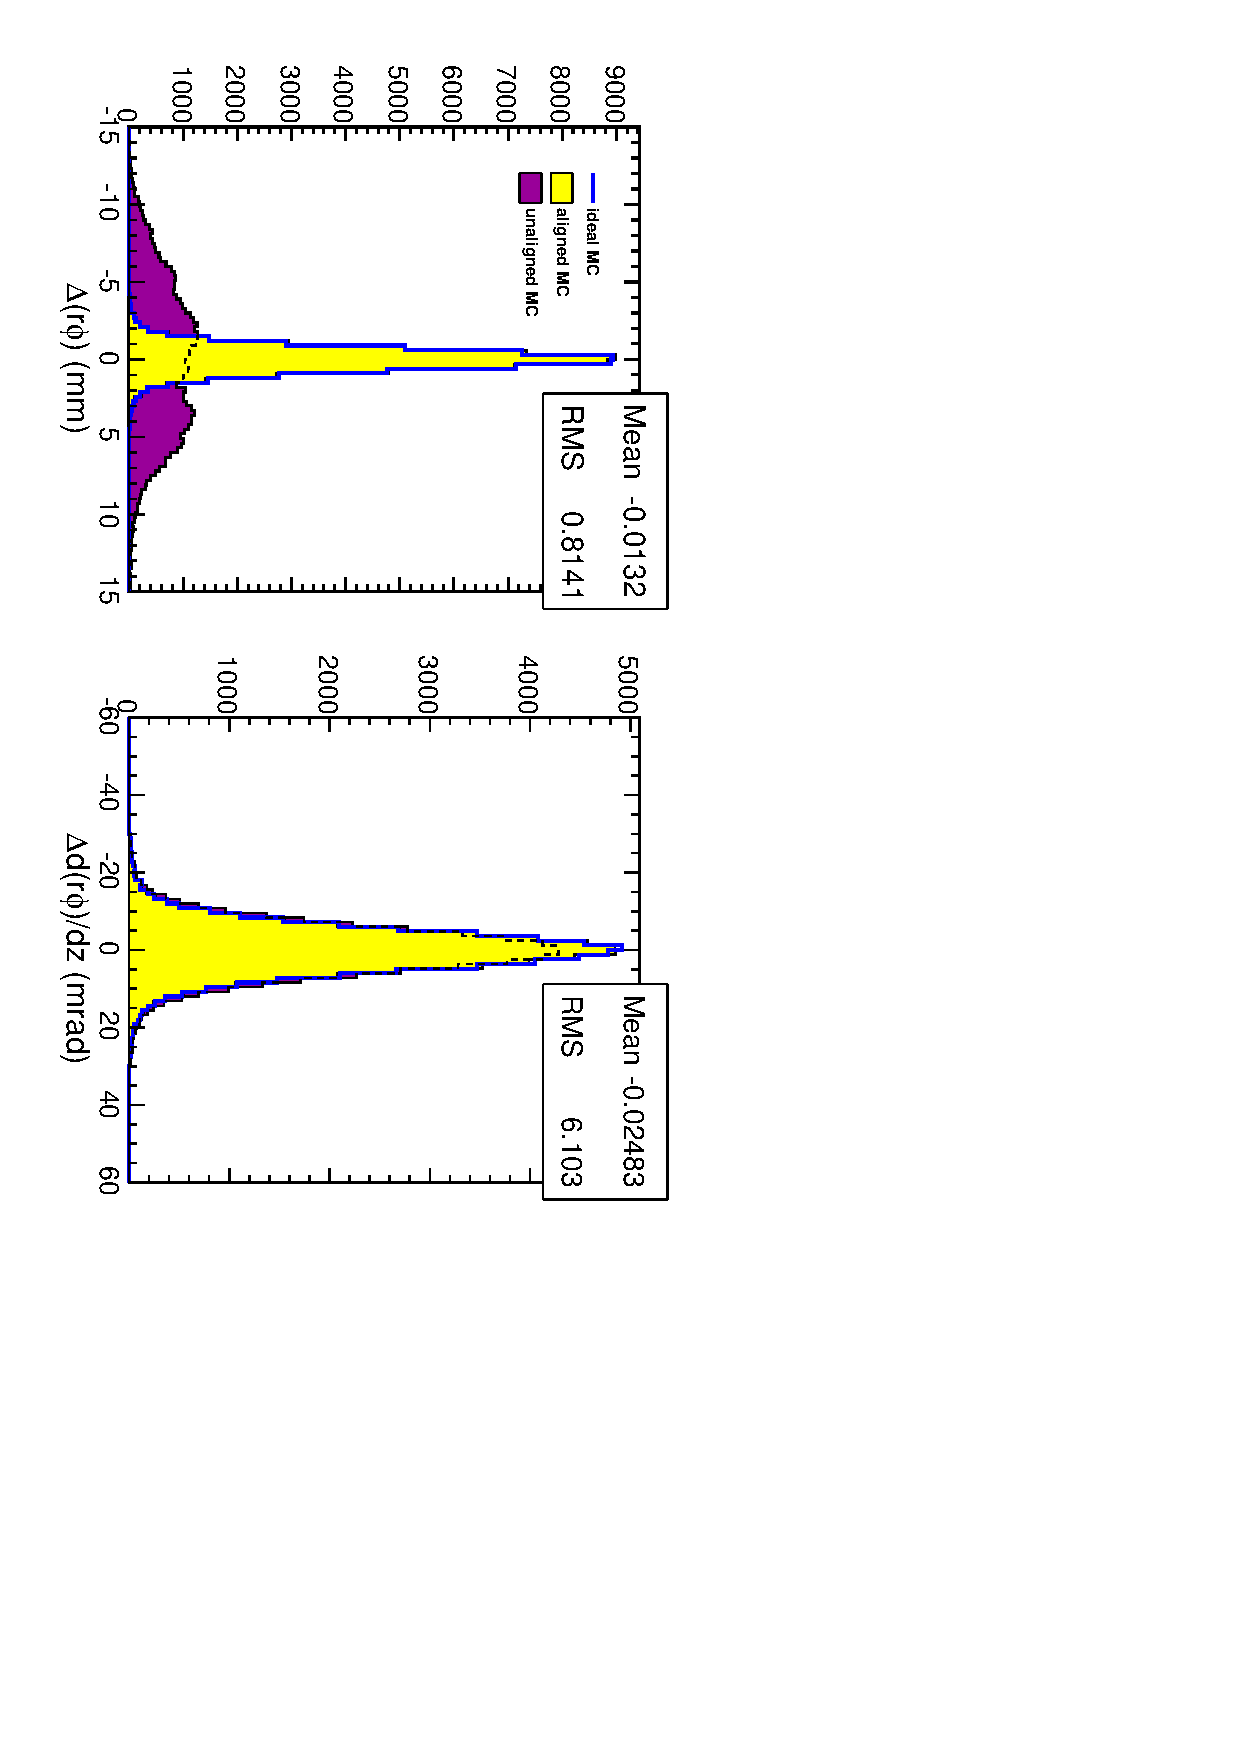
\includegraphics[height=0.8\linewidth, angle=90]{residuals.pdf}
\end{center}

\vfill
\begin{itemize}
\item Toy MC $\Delta \frac{d(r\phi)}{dz}$ distribution is 2~mrad wide: need to find out what is different in the full MC (potential for improvement?)
\item Tracker-to-CSC $\Delta \frac{d(r\phi)}{dz}$ distribution is 5~mrad wide; the above is slightly narrower, accounting for $\sqrt{2}$
\item 6~mrad $\Delta \frac{d(r\phi)}{dz}$ distribution implies 0.76~mm $\Delta (r\phi)$ distribution, so the above is consistent with intercepts dominated by slope error
\end{itemize}
\end{frame}

\begin{frame}
\frametitle{Closure tests}
\begin{itemize}
\item $\displaystyle \sum_i^{18} \Delta (r\phi)_i$ and $\displaystyle \sum_i^{18} \Delta \frac{d(r\phi)}{dz}_i$ must both be zero
\item Independent of alignment: tests consistency of residuals
\item MC results (sum over chambers, not average):
\end{itemize}

\begin{center}
\renewcommand{\arraystretch}{1.2}
\begin{tabular}{c | c c}
ring & $\Delta (r\phi)$ (mm) & $\Delta \frac{d(r\phi)}{dz}$ (mrad) \\\hline
ME+4/1 & $-0.13 \pm 0.33$ & $-4.6 \pm 2.0$ \\
ME+3/1 & $-0.41 \pm 0.22$ & $0.1 \pm 1.5$ \\
ME+2/1 & $0.02 \pm 0.19$ & $2.4 \pm 1.2$ \\
ME$-$2/1 & $-0.26 \pm 0.19$ & $1.6 \pm 1.17$ \\
ME$-$3/1 & $-0.05 \pm 0.23$ & $-3.4 \pm 1.5$ \\
ME$-$4/1 & $0.01 \pm 0.32$ & $-3.4 \pm 2.2$ \\
\end{tabular}
\end{center}
\end{frame}

\begin{frame}
\frametitle{Patch for incomplete rings}

\begin{itemize}\setlength{\itemsep}{0.25 cm}
\item New feature: can align incomplete rings by {\it assuming}
\begin{center}
$\displaystyle \sum_i^N \Delta (r\phi)_i = 0$ \hspace{0.5 cm}and\hspace{0.5 cm} $\displaystyle \sum_i^N \Delta \frac{d(r\phi)}{dz}_i = 0$
\end{center}

\item Closure test is no longer available as a cross-check

\item Only works for certain topologies:
\end{itemize}

\vfill
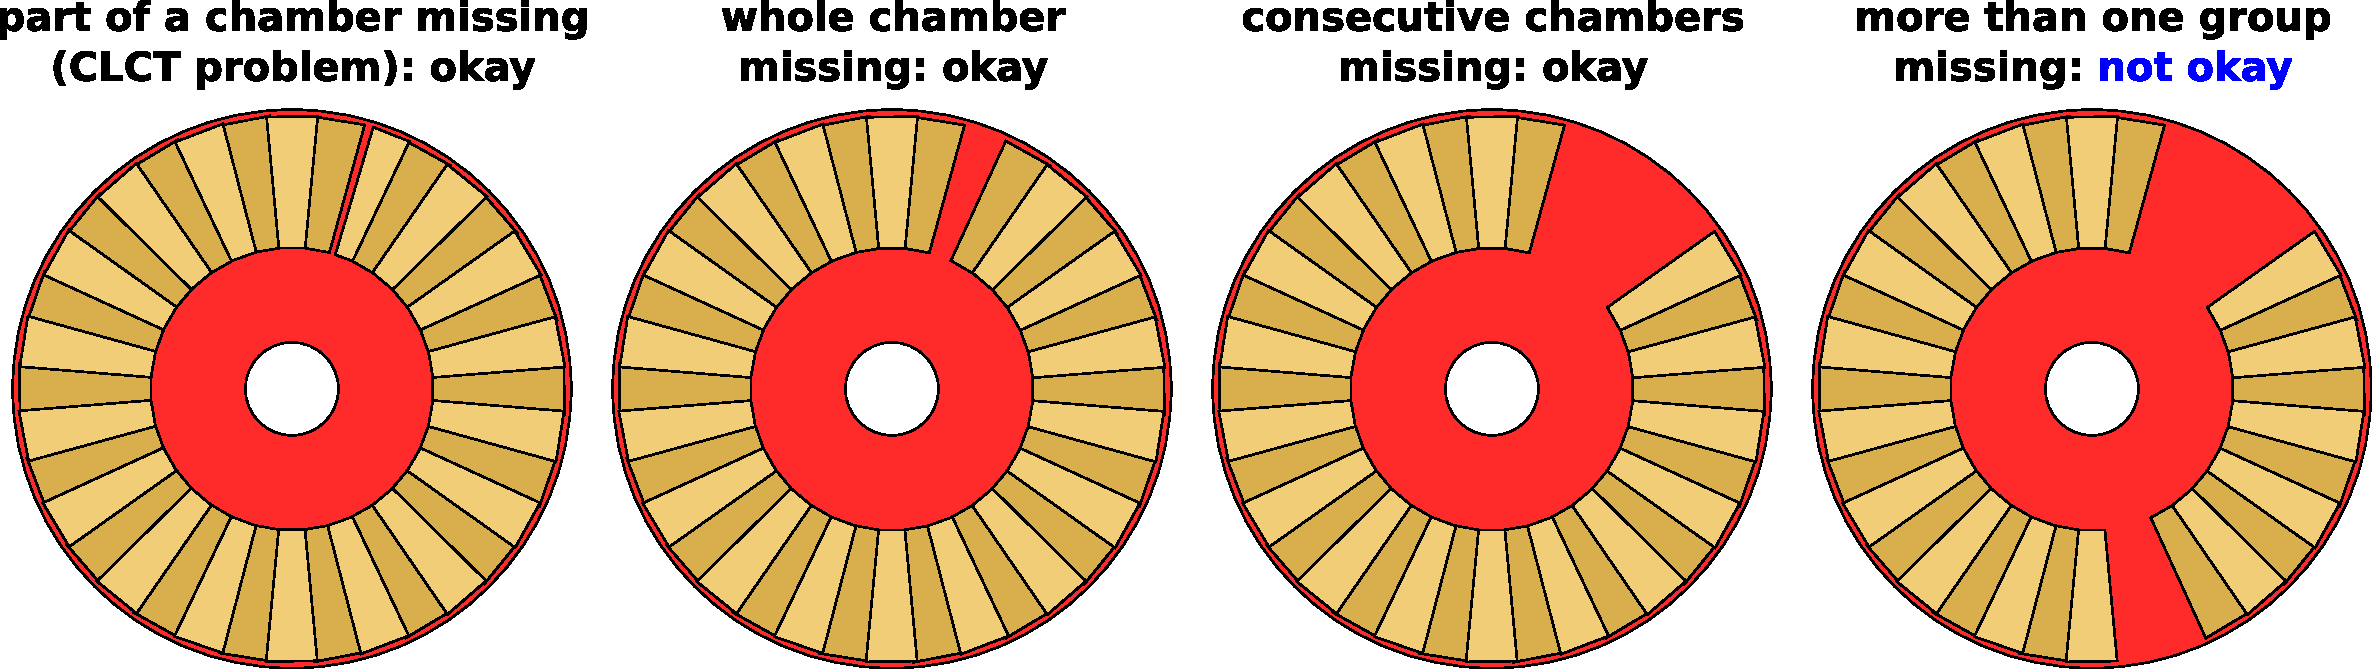
\includegraphics[width=\linewidth]{incomplete_rings.pdf}
\end{frame}

\begin{frame}
\frametitle{Low-statistics rings}

\vfill
\begin{columns}
\column{0.7\linewidth}
\textcolor{darkblue}{ME$\pm$1/1b (complete with $N_{\mbox{\scriptsize hits}} \ge 5$)}
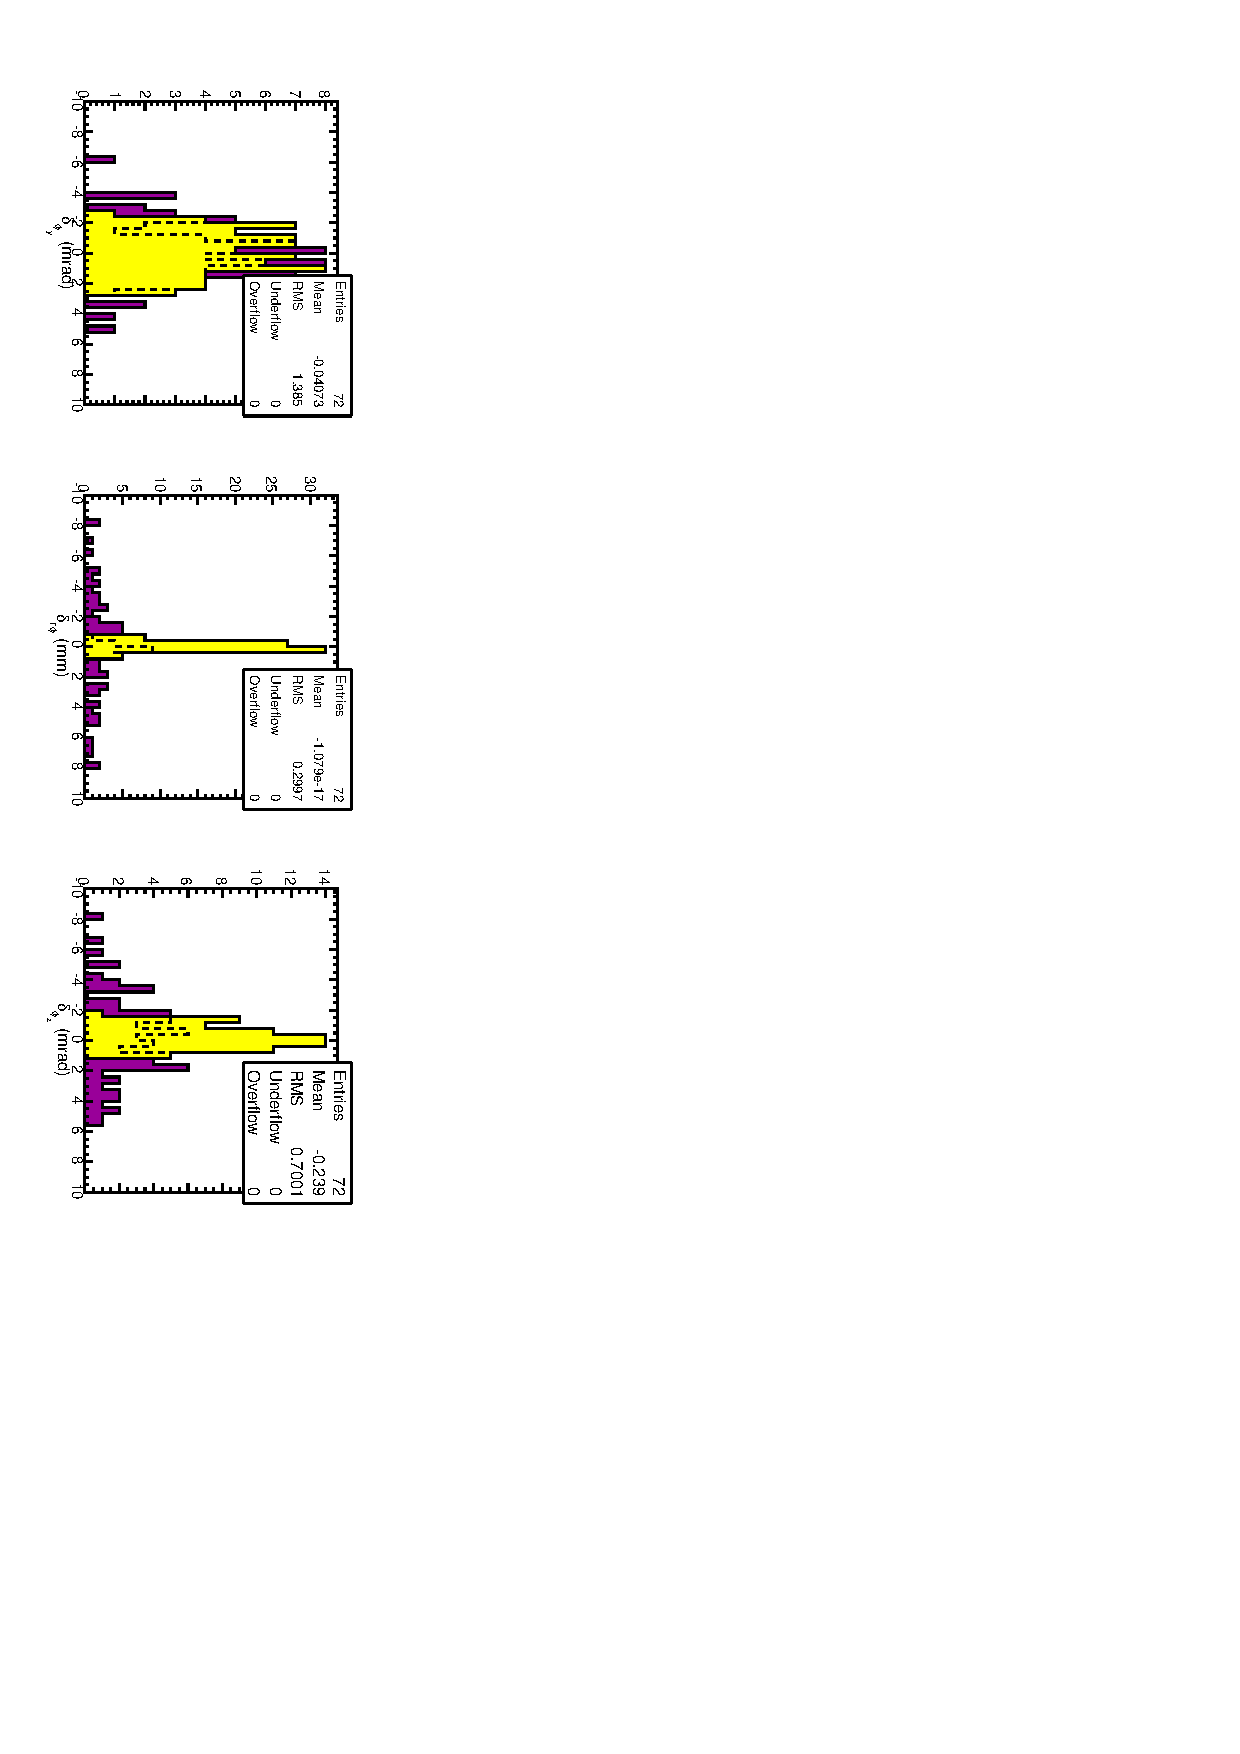
\includegraphics[height=\linewidth, angle=90]{alignall_me11b.pdf}

\vspace{0.2 cm}
\textcolor{darkblue}{ME$\pm$1/2 (complete with $N_{\mbox{\scriptsize hits}} \ge 5$)}
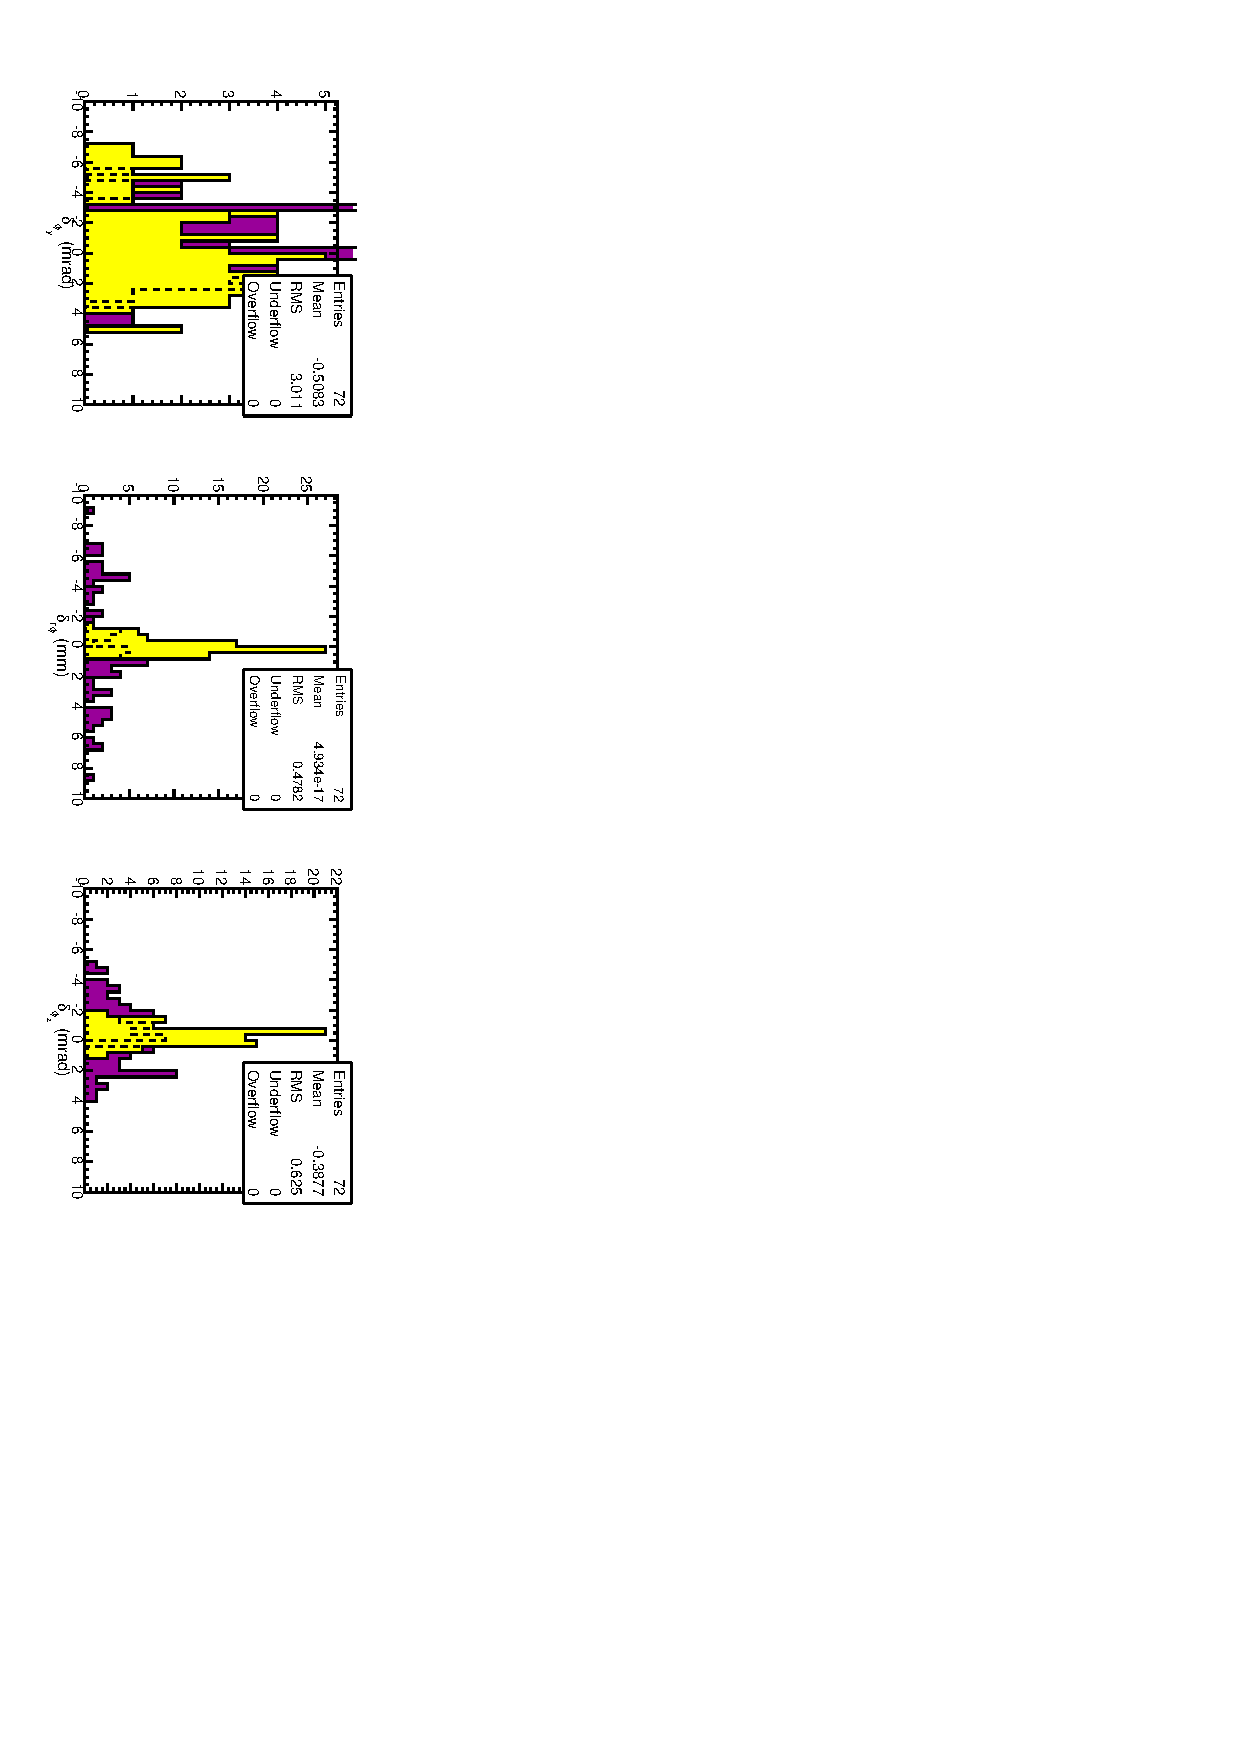
\includegraphics[height=\linewidth, angle=90]{alignall_me12.pdf}

\vspace{0.2 cm}
\textcolor{darkblue}{ME$\pm$2/2 and ME$-$3/2 (all incomplete, fix $\phi_y$)}
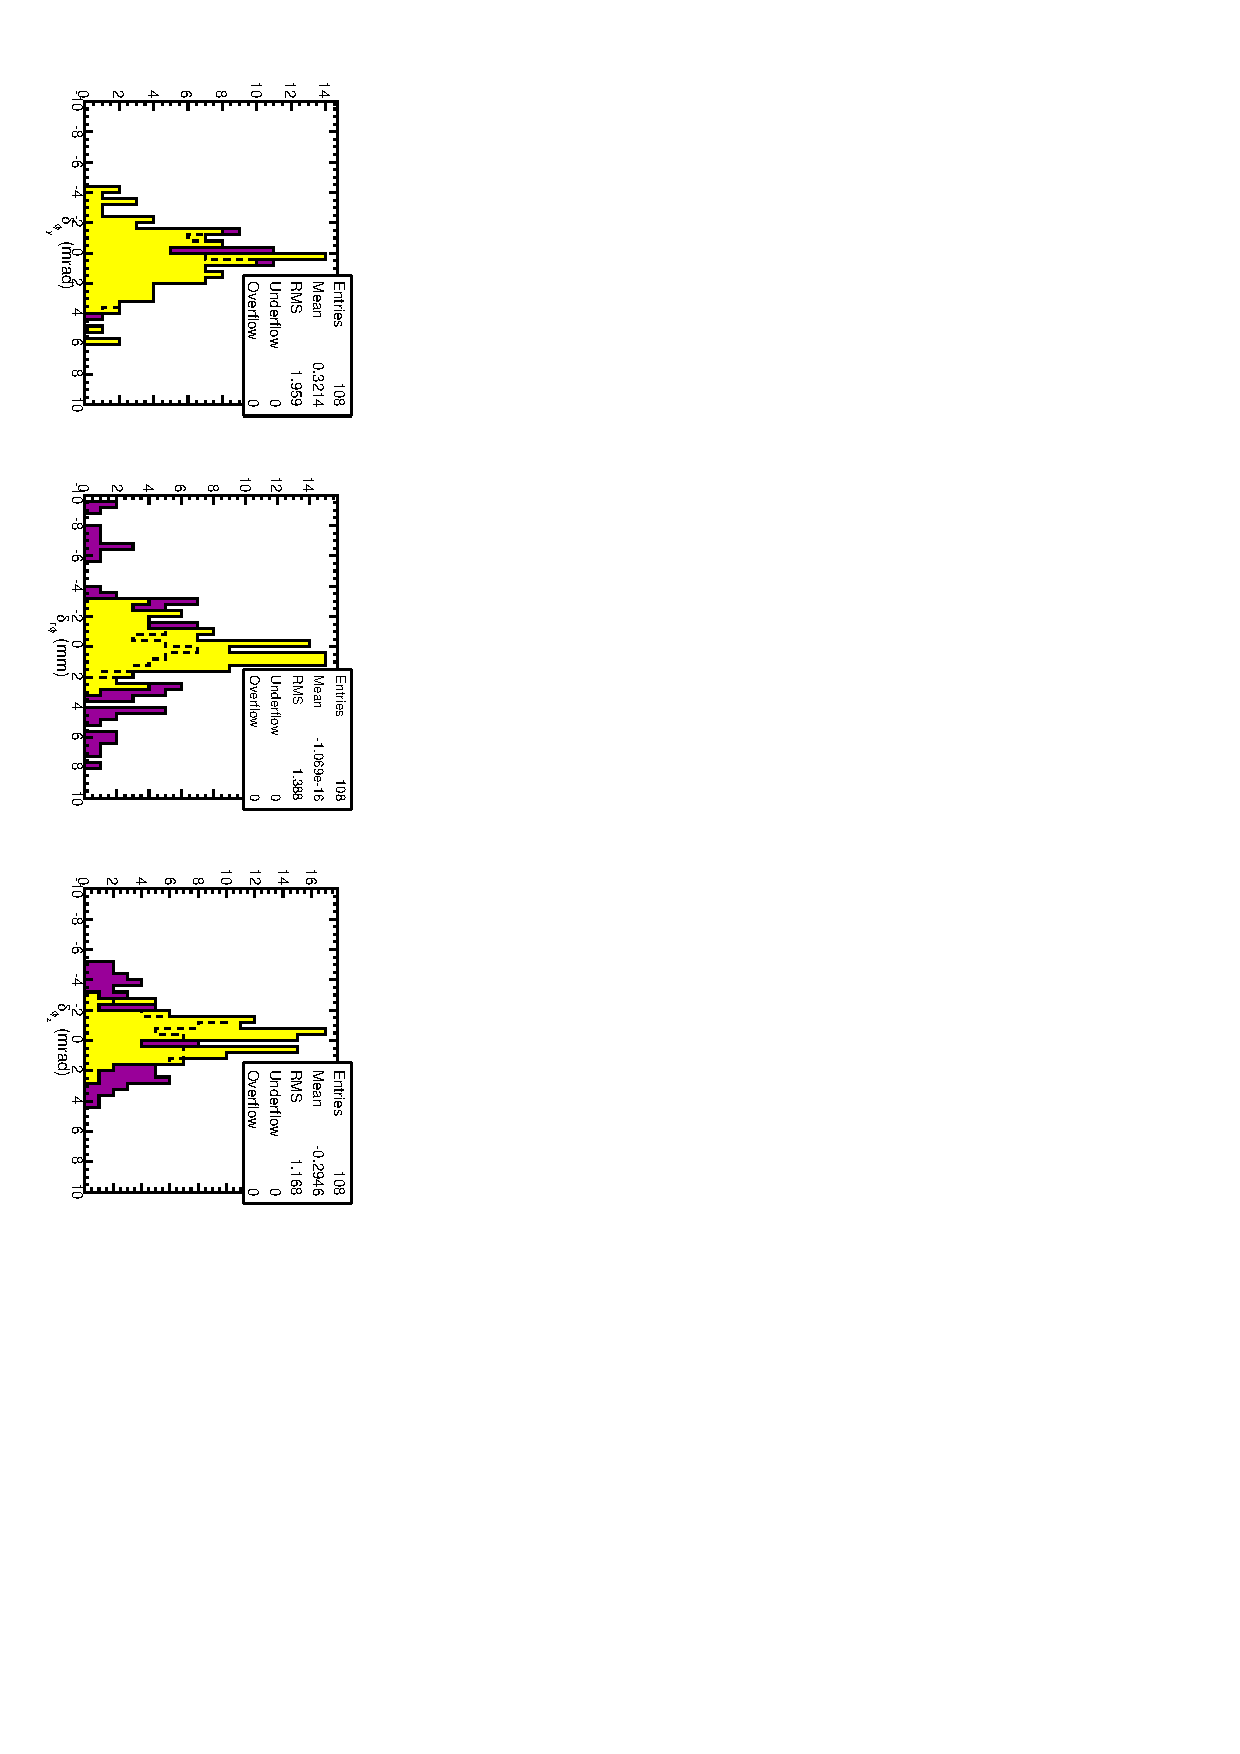
\includegraphics[height=\linewidth, angle=90]{skipphiy_me22_mem32.pdf}
\column{0.3\linewidth}

\begin{itemize}
\item Lowered $N_{\mbox{\scriptsize hits}}$ threshold to 5 to align more rings
\item ME2/2, 3/2 \mbox{(far from beamline)} are incomplete, but only $+$3/2 is missing multiple groups
\item Alignment in ME2/2, 3/2 only possible by fixing $\phi_y$ (due to low statistics)
\item Roughly 1/2 hour of circulating beam
\end{itemize}
\end{columns}
\end{frame}


%% \begin{frame}
%% \frametitle{Outline}
%% \begin{itemize}\setlength{\itemsep}{0.75 cm}
%% \item 
%% \end{itemize}
%% %% \hspace{-0.83 cm} \textcolor{darkblue}{\Large Outline2}
%% \end{frame}

%% \section*{First section}
%% \begin{frame}
%% \begin{center}
%% \Huge \textcolor{blue}{First section}
%% \end{center}
%% \end{frame}

\begin{frame}
\frametitle{Conclusions}
\begin{itemize}\setlength{\itemsep}{0.5 cm}
\item Last year's software still works, with a minor update
\item New occupancy plots help to monitor trigger/read-out issues
\item Added ability to align incomplete rings, for some topologies
\item Need to combine ME1/1a and 1/1b chambers, especially if 1/1a is shadowed by trigger geometry
\end{itemize}
\label{numpages}
\end{frame}

\end{document}
